\documentclass[12pt,a4paper]{article}
% Internationalization 
\usepackage[utf8]{inputenc}
% Better hyphenation for words with digraphs čćžšđ
\usepackage[T1]{fontenc} 
% Set Croatian as active language
\usepackage[croatian]{babel}
% For importing images - .jpg, .png, .pdf, .svg, .eps
\usepackage{graphicx}
% For manualy figure postioning
\usepackage{float} 
% For adding colors to text
\usepackage{color}
% Enabling more defined colors
\usepackage[usenames,dvipsnames]{xcolor}
% Support for .txt listings w/o begin{verbatim}
\usepackage{listings} 
% Pro­vides diffrent formats for \today
\usepackage{datetime}
% For Toc with dots
\usepackage{tocloft} 
% Define geometry
\usepackage[left=2.5cm,top=2.5cm,right=2cm,bottom=2.5cm]{geometry} 
% For fancy headers and footers
\usepackage{fancyhdr} 
% For adding Bibliography in TOC
\usepackage[nottoc]{tocbibind} 
% LaTex has support for simple math formulas 
% For advance mathematical formulas we use
\usepackage{amsmath}
% For setting line spacing e.g. \dobulespacing
\usepackage{setspace}
% Simplifies including multi-page PDF or PS docs
\usepackage{pdfpages}
% For changing title styls with \titleformat
\usepackage[explicit]{titlesec}

% Fancy header definition
\pagestyle{fancy}
% Removes default rule in header
\renewcommand{\headrulewidth}{0pt} 
\fancyhf{}
% Set page number in down-right corner of the page
\rfoot{\thepage}

% Change figure name prefix - has to be before \begin{document}
\addto\captionscroatian{\renewcommand{\figurename}{Sl.}}

\begin{document}

% Change section, subsection figure, table. listing numbering
\renewcommand{\thesection}{\arabic{section}.}
\renewcommand{\thesubsection}{\arabic{section}.\arabic{subsection}.}
\renewcommand{\thefigure}{\arabic{section}.\arabic{figure}.} 
\renewcommand{\thetable}{\arabic{section}.\arabic{table}.}
\renewcommand{\thelstlisting}{\arabic{section}.\arabic{lstlisting}.} 

% Change section format style
\titleformat{\section}
  {\Large\bfseries}{\thesection}{1em}{\MakeUppercase{#1}}

% Change listing name
\renewcommand\lstlistingname{Ispis koda} 
\renewcommand\lstlistlistingname{Ispis koda}

\definecolor{myyellow}{HTML}{FFB902}
\definecolor{mygreen}{HTML}{009B57}
\definecolor{myred}{HTML}{D13D29}
\definecolor{myblue}{HTML}{1469EA}

\lstset{ %
    backgroundcolor=\color{white},   
    basicstyle=\footnotesize,        
    breakatwhitespace=false,         
    breaklines=true,                 
    % captionpos=b,                    
    commentstyle=\color{mygreen},    
    deletekeywords={...},            
    escapeinside={\%*}{*)}, 
    extendedchars=true,              
    frame=single,                    
    keepspaces=true,                 
    keywordstyle=\color{myblue},       
    keywordstyle=[2]\color{myred},
    language=C,
    morekeywords={new},            
    keywords=[2]{pcl, PCLPointCloud2, ptr, PCDReader, PCDWriter},
    numbers=left,                    
    numbersep=5pt,                   
    numberstyle=\tiny\color{myyellow}, 
    rulecolor=\color{black},         
    showspaces=false,                
    showstringspaces=false,          
    showtabs=false,                  
    stepnumber=2,                    
    stringstyle=\color{myred},     
    tabsize=2,                       
    title=\lstname                   
}

\newpage
\begin{titlepage}
\begin{center}

\textbf{\MakeUppercase{\large 
    Sveučilište Josipa Jurja Strossmayera u Osijeku}}\\[0.2cm]

\textbf{\MakeUppercase{\large Elektrotehnički fakultet}}\\[0.8cm]
\textbf{\large Sveučilišni studij}\\ [5cm]

\textbf{\MakeUppercase{\Large 
    Izgradnja 3D modela scene pomoću 3D kamere }}\\ [1cm]

\textbf{\large Diplomski rad}\\  [5 cm] 

\textbf{\Large Marijan Svalina}\\ [0.5cm] 

\vfill

\textbf{\large Osijek, 2013.} \\

\end{center}
\end{titlepage}

% \includepdf[pages={1}]{Obrazac_Z1_04.pdf}
% \includepdf[pages={1}]{izjava_o_originalnosti}
\newpage
% Toc  
\renewcommand{\cftsecleader}{\cftdotfill{\cftdotsep}}
\tableofcontents 
% Removing page numbering from this page 
\thispagestyle{empty}

\newpage

\setcounter{page}{1}
\setcounter{figure}{0}
\section{Uvod}% (fold)
\label{sec:Uvod}

\subsubsection{Zadatak diplomskog rada} % (fold)
\label{ssub:Zadatak diplomskog rada}

Program RGBDSLAM raspoloživ u okviru programske biblioteke OpenSLAM
omogućava izgradnju 3D modela objekata i scena pomoću 3D kamere.
Razviti program za izgradnju 3D modela u obliku mreže trokuta koristeći
biblioteku PointCloud. Kombinacijom ova dva programa mogu se izgraditi
3D modeli objekata i scena snimljenih iz više pogleda. Zadatak je
ispitati funkcionalnost navedenog postupka kao i kvalitetu dobivenog
rezultata izgradnjom nekoliko 3D modela objekata i scena.

% subsubsection Zadatak diplomskog rada (end)
% section Uvod (end)

\newpage
\setcounter{figure}{0}

\section{Pregled korištenih tehnologija i algoritama} % (fold)
\label{sec:Tehnologija i teorija}

\subsection{Microsof Kinect 3D kamera} % (fold)
\label{sub:Microsof Kinect 3D kamera}

Kinect je RGB-D senzor koji daje sliku u boji sinkroniziranu s dubinskom
slikom. Inicijalno je korišten kao ulazni uređaj za Microsoft Xbox
igračku konzolu. Algoritmima za prepoznavanje ljudskih pokreta omogućava
interakciju između igre i igrača bez potrebe za korištenjem kontrolera.
Nakon pojave senzora zajednica znanstvenika koji proučavaju računalni
vidi otkrila je da tehnologija korištena za dohvaćanje dubine može biti
upotrebljena za puno više od igranja za puno manje cijenu nego
tradicionalne 3D kamere kao što su stereo i Time-of-flight kamere.

Dodatno, komplementarna priroda informacije o dubine na slici koju pruža
Kinect olakšava nova potencijalna rješenja klasičnih problema računalnog
vida. U samo dvije godine nakon puštanja u prodaju Kinecta, velik broj
znanstvenih članaka i demonstracija se pojavio na raznim konferencijama.

\begin{figure}[h]
\centering
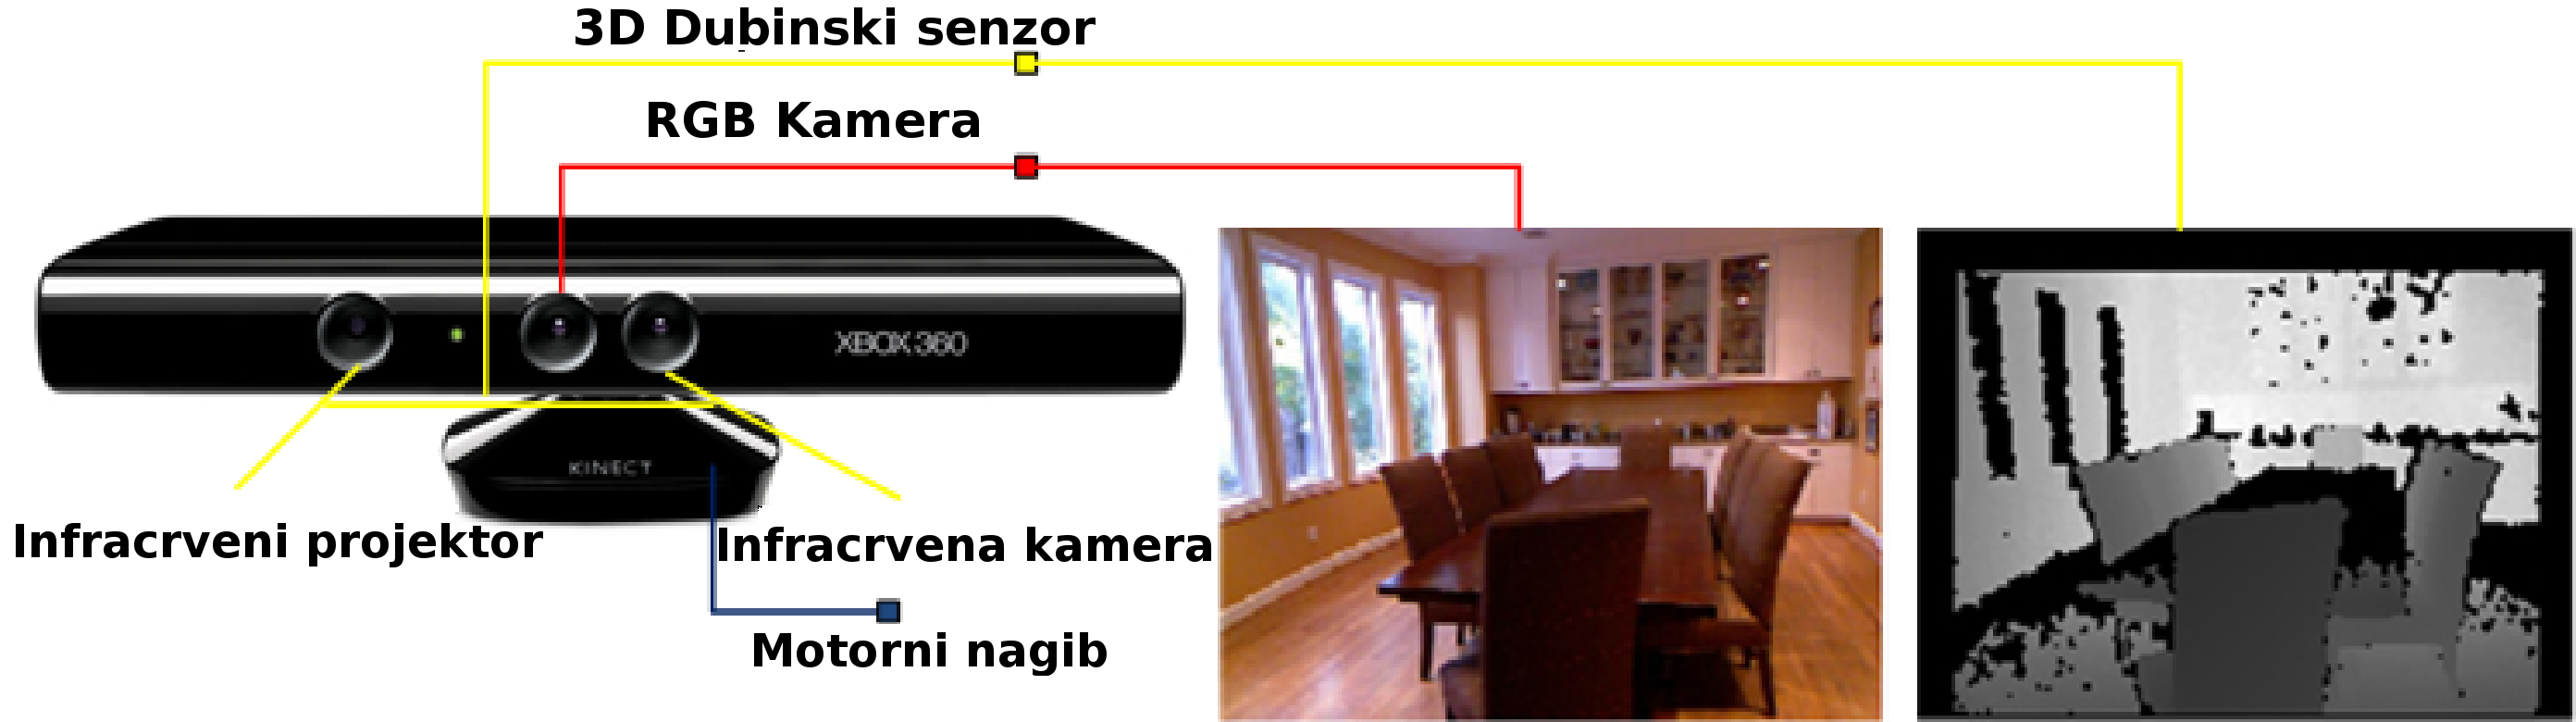
\includegraphics[scale=0.15]{figures/kinect.png}
\caption{Shematski prikaz Kinect kamere, izvor:~\cite{HanSXS13}}
\label{fig:kinect.png}
\end{figure}

\subsubsection{Tehničke specifikacije} % (fold)
\label{ssub:Tehničke specifikacije}

Slika~\ref{fig:kinect.png} prikazuje raspored Kinect senzora. Kinect se
sastoji od infracrevnog (IR) projektora, IR kamere i RGB kamere.
Dubinski senzor se sastoji od IR projektora i IR kamere. IR projektor
projicira IR uzorak točkastih mrlja na 3D scenu dok IR kamera hvata
reflektirane IR mrlje. Kinect radi na principu strukturirane svjetlosti.
Geometrijska veza između IR projektora i IR kamere se ostvaruje offline
kalibracijskom procedurom. IR projektor projicira poznat uzorak
svjetlosnih mrlja na scenu. IR svjetlost je nevidljiva RGB kameri ali
je vidljiva IR kameri. Kako je svaki lokalni uzorak projiciranih točaka
jedinstven, spajanje promatranih lokalnih uzoraka točaka sa slike
s kalibriranim projektorovim uzorkom točaka je ostvarivo. Više o
principu strukturirane svjetlosti u~\cite{structured:light}.\\

Tehničke informacije o kameri:
\begin{itemize}
    \item \textbf{RGB kamera} daje sliku rezolucije \(640\times480\)
        piksela pri osvježavanju slike od 30Hz. Postoji i opcija davanja
        slike rezolucije \(1280 \times 1024\) piksela ali se dobije samo 10
        sličica po sekundi.
    \item \textbf{3D Dubinski senzor} se sastoji od IR laserskog
        projektora i IR kamere. Zajedno, projektor i kamera kreiraju
        dubinsku mapu, koja pruža informaciju o udaljenosti između
        objekta i kamere. Senzor ima praktično ograničenje u dometu 
        0.8m - 3.5m. Kamera daje video od 30 sličica po sekundi s
        rezolucijom \(640 \times 480\) piksela. Vidno polje senzora je
        \(57\,^{\circ}\) horizontalno i \(43\,^{\circ}\) vertikalno.
    \item \textbf{Motorni nagib} upravlja nagibom Kinecta. Nagib može
        biti pomaknuti \(27\,^{\circ}\) gore ili dolje.
\end{itemize}

% subsubsection Tehničke specifikacije (end)

% subsection Microsof Kinect 3D kamera (end)

\newpage
\subsection{ROS biblioteka i alati} % (fold)
\label{sub:ROS biblioteka i alati}

ROS~\cite{ros} (engl. \textit{Robot Operating System}) je set programskih
biblioteka i alata koji pomažu programerima kreirati aplikacije za
robote. Pruža hardversku abstrakciju, upravljačke programe, biblioteke,
vizualizaciju, komunikaciju, upravljanje paketima i dr. ROS je
licenciran BSD licencom, koja spada pod licence otvorenog koda.

\begin{figure}[h]
\centering
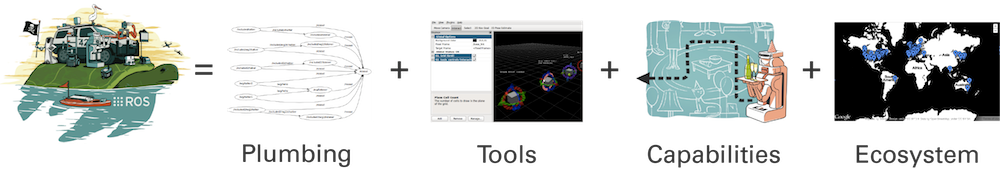
\includegraphics[scale=0.45]{figures/ros.png}
\caption{Shematski prikaz ROSa}
\label{fig:ros.png}
\end{figure}

U ovom radu ROS se dotiče kroz program RGBDSlam koji je opisan u
potpoglavlju~\ref{sub:Snimanje scene 3D kamerom i RGBDSlam programom} te se oslanja na
njegove biblioteke, upravljačke programe i alate. Tako RGBDSlam koristi
OpenNI upravljački program za komunikaciju s Kinect kamerom u obliku ros
programskog paketa (\texttt{ros-fuerte-openni-launch}). Također, RGBDSlam
koristi i niz drugih paketa iz ROS biblioteke~\cite{web:rgbdslam}

% subsection ROS biblioteka i alati (end)

\subsection{Biblioteka Pointcloud} % (fold)
\label{sub:Biblioteka Pointcloud}

PCL~\cite{pcl} (engl. \textit{Point Cloud Library}
slika~\ref{fig:pcl.png}) je otvoren projekt za procesiranje 2D/3D slika
i oblaka točaka. PCL biblioteka sadržava niz najsuvremenijih algoritama
za filtriranje, estimaciju značajki, rekonstrukciju površina,
registraciju, uklapanje modela i segmentaciju.  Ti algoritmi se mogu
koristiti npr. za izbacivanje odudarajućih vrijednosti iz šumovith
podataka, spajanje 3D oblaka točaka, segementiranje relevantnih dijelova
scene, izvlačenje ključnih točaka i računanje deskriptora za
prepoznavanje objekata na temelju njihove geometrije, kreiranje i
prikazivanje površina iz oblaka točaka itd.

\begin{figure}[h]
\centering

\includegraphics[scale=0.15]{figures/pcl.png}
\caption{PCL logo}
\label{fig:pcl.png}
\end{figure}

PCL je objavljen pod BSD licencom i softver je otvorenog koda. Što znači
da je slobodan za upotrebu u komercijalne i akademske svrhe.

PCL se uspješno prevodi na GNU/Linux, MacOS, Windows i Android/iOS
platformama. Zbog olakšanog razvijanja podijeljen je na više manjh
biblioteka koje se mogu prevoditi zasebno. PCL se može prikazati kao
graf biblioteka kao što je prikazano na slici~\ref{fig:pcl-graph.png}

\begin{figure}[h]
\centering
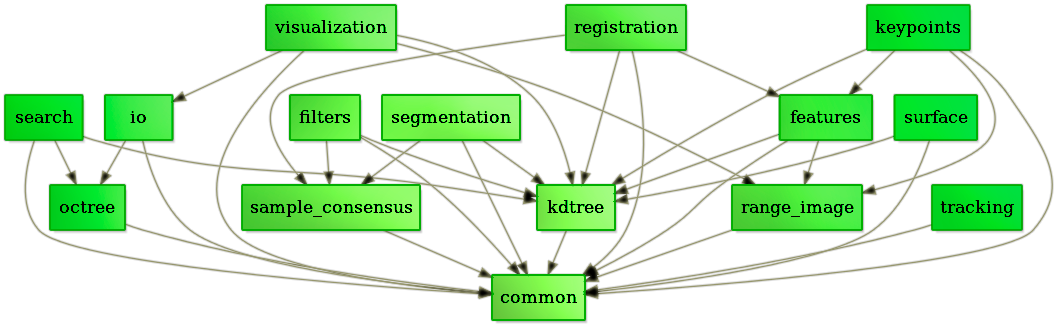
\includegraphics[scale=0.40]{figures/pcl-graph.png}
\caption{Graf PCL biblioteka}
\label{fig:pcl-graph.png}
\end{figure}

% subsection Biblioteka Pointcloud (end)


\newpage
\subsection{Istovremena lokalizacija i mapiranje} % (fold)
\label{sub:Slam}
Jedno od najznačajnijih područja istraživanja na polju mobilne robotike
su metode istovremene lokalizacije i mapiranja
(engl.\textit{Simultaneous Localization and Mapping} - SLAM). SLAM su
originalno razvili Hugh Durrant-Whyte i John J.
Leonard~\cite{Durrant:91b} koji su rad bazirali na prethodnom radu
Smitha, Selfa and Cheesemana~\cite{Smith86}. SLAM se bavi rješavanjem
problema izgradnje mape nepoznate okoline mobilnog robota te istovremeno
navigiranje robota okolinom koristeći tu mapu.

SLAM se sastoji iz nekoliko koraka: izvlačenja orijentira, pridruživanja
podataka, estimiranja stanja, ažuriranja stanja i ažuriranja orijentira.
Postoji više načina kako realizirati svaki od tih koraka. SLAM se može
primjeniti na 2D i 3D kretanje.

\subsubsection{Osnovna ideja i kratak pregled koraka} % (fold)
\label{ssub:Osnovna ideja }
Proces istovremene lokalizacije i mapiranja se sastoji iz nekoliko
koraka. Cilj procesa je koristiti precepciju okolinu za ažuriranje pozicije robota.
Zbog nesavršenosti odometrije robota nije dobro osloniti se samo na nju
kako bi se pronašla pozicija robota već se može koristiti lasersko
skeniranje okoline ili, kao u slučaju RGBDSlam programa, Kinect 3D kamera
kako bi pronašli pravu poziciju robota/kamere. To se postiže
detekcijom značajki u okolini i promatranjem tih značajki kada se
robot pomakne. EKF (\textit{Extended Kalman Filter}) prošireni Kalmanov
filter je jezgra SLAM procesa. EKF je odgovoran za ažuriranje pozicije
na kojoj robot ``misli'' da se nalazi koristeći izvučene značajke. Takve
značajke se još nazivaju i orijentiri. EKF prati estimaciju nesigurnosti
pozicije robota i nesigurnosti orijentira iz okoline. Pregled SLAM
procesa~\footnotemark[1] se nalazi na grafikonu~\ref{fig:slam-overview.pdf}  

\footnotetext[1]{%
Grafikon je inspiriran sličnim grafikonom iz rada SLAM for
Dummies~\cite{web:slam} }

\begin{figure}[h]
\renewcommand{\figurename}{Grafikon}
\centering
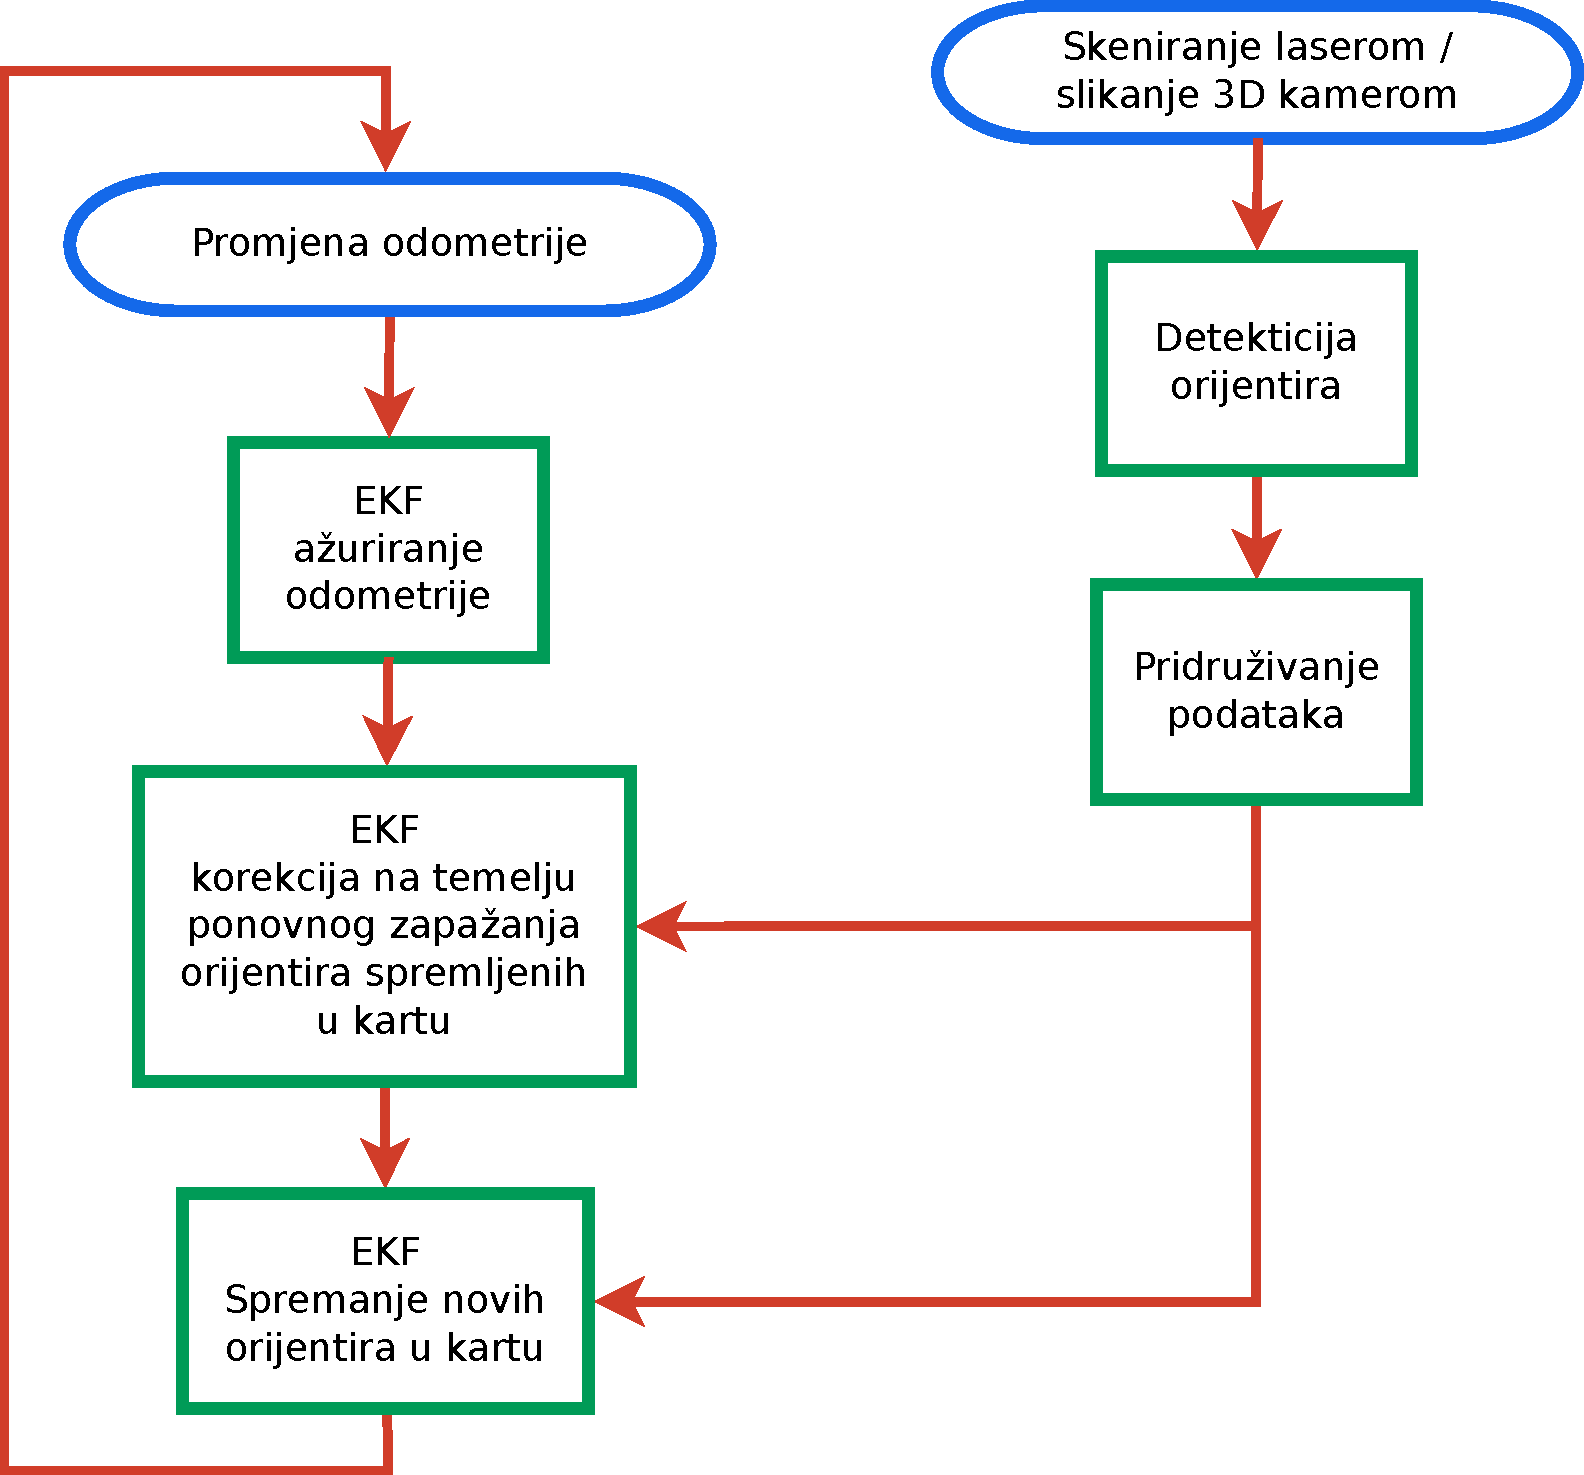
\includegraphics[scale=0.4]{figures/slam-overview.pdf}
\caption{Pregled SLAM procesa}
\label{fig:slam-overview.pdf}
\end{figure}

Kad se odometrija promijeni zato što se robot pomakao, nesigurnost koja se
tiče robotove nove pozicije se ažurira u EKF koristeći ažuriranje
odometrije. Orijentiri se tada detektiraju u okoline iz robotove nove
pozicije. Robot tada pokušava asocirati detektirane orijentire s prije zapaženim
orijentirima spremljenim u kratu. Ponovno zapaženi orijentiri se tada koriste za ažuriranje
pozicije robota u EKFu. Orijentiri koji prije nisu zapaženi se dodaju u
kartu kako bih se mogli koristiti kasnije. U svakom od opisanih koraka EKF
računa estimaciju robotove trenutne pozicije. 

\subsubsection{Proširen Kalmanov filter - EKF} % (fold)
\label{ssub:Proširen Kalmanov filter - EKF}

Kalmanov filter je algoritam koji koristi niz mjerenja pribavljenih
tijekom vremena, koja sadržavaju šum i ostale netočnosti, te računa
estimacije nepoznatih varijabli koje su, u slučaju zadovoljenja
pretpostavki algoritma, preciznije od računa baziranom samo na jednom
mjerenju. Konkretnije, Kalmanov filter se izvršava rekurzivno na nizu
šumovith ulaznih podataka i računa statistički optimalnu estimaciju
sustava stanja. Filter je nazvan po Rudolfu E. Kalmanu~\cite{Kalman}
koji je jedan od primarnih razvijatelja teorije.


Algoritam je podijeljen u dva koraka kao što se vidi na
grafikonu~\ref{fig:basic-kalman}. U prvom predikcijskom koraku Kalmanov
filter računa estimaciju trenutnih varijabla stanja s njihovim
nesigurnostima na temelju modela kretanja robota. U drugom korekcijskom
koraku, kada je promotren rezultat sljedećeg mjerenja (koje isto ima
greške pri mjerenju i šum mjerenja), izračunata estimacija se korigira
upotrebom težinske sredine gdje se više težine daje estimaciji s većom
vjerojatnošću.

\begin{figure}[h]
\centering
\renewcommand{\figurename}{Grafikon}
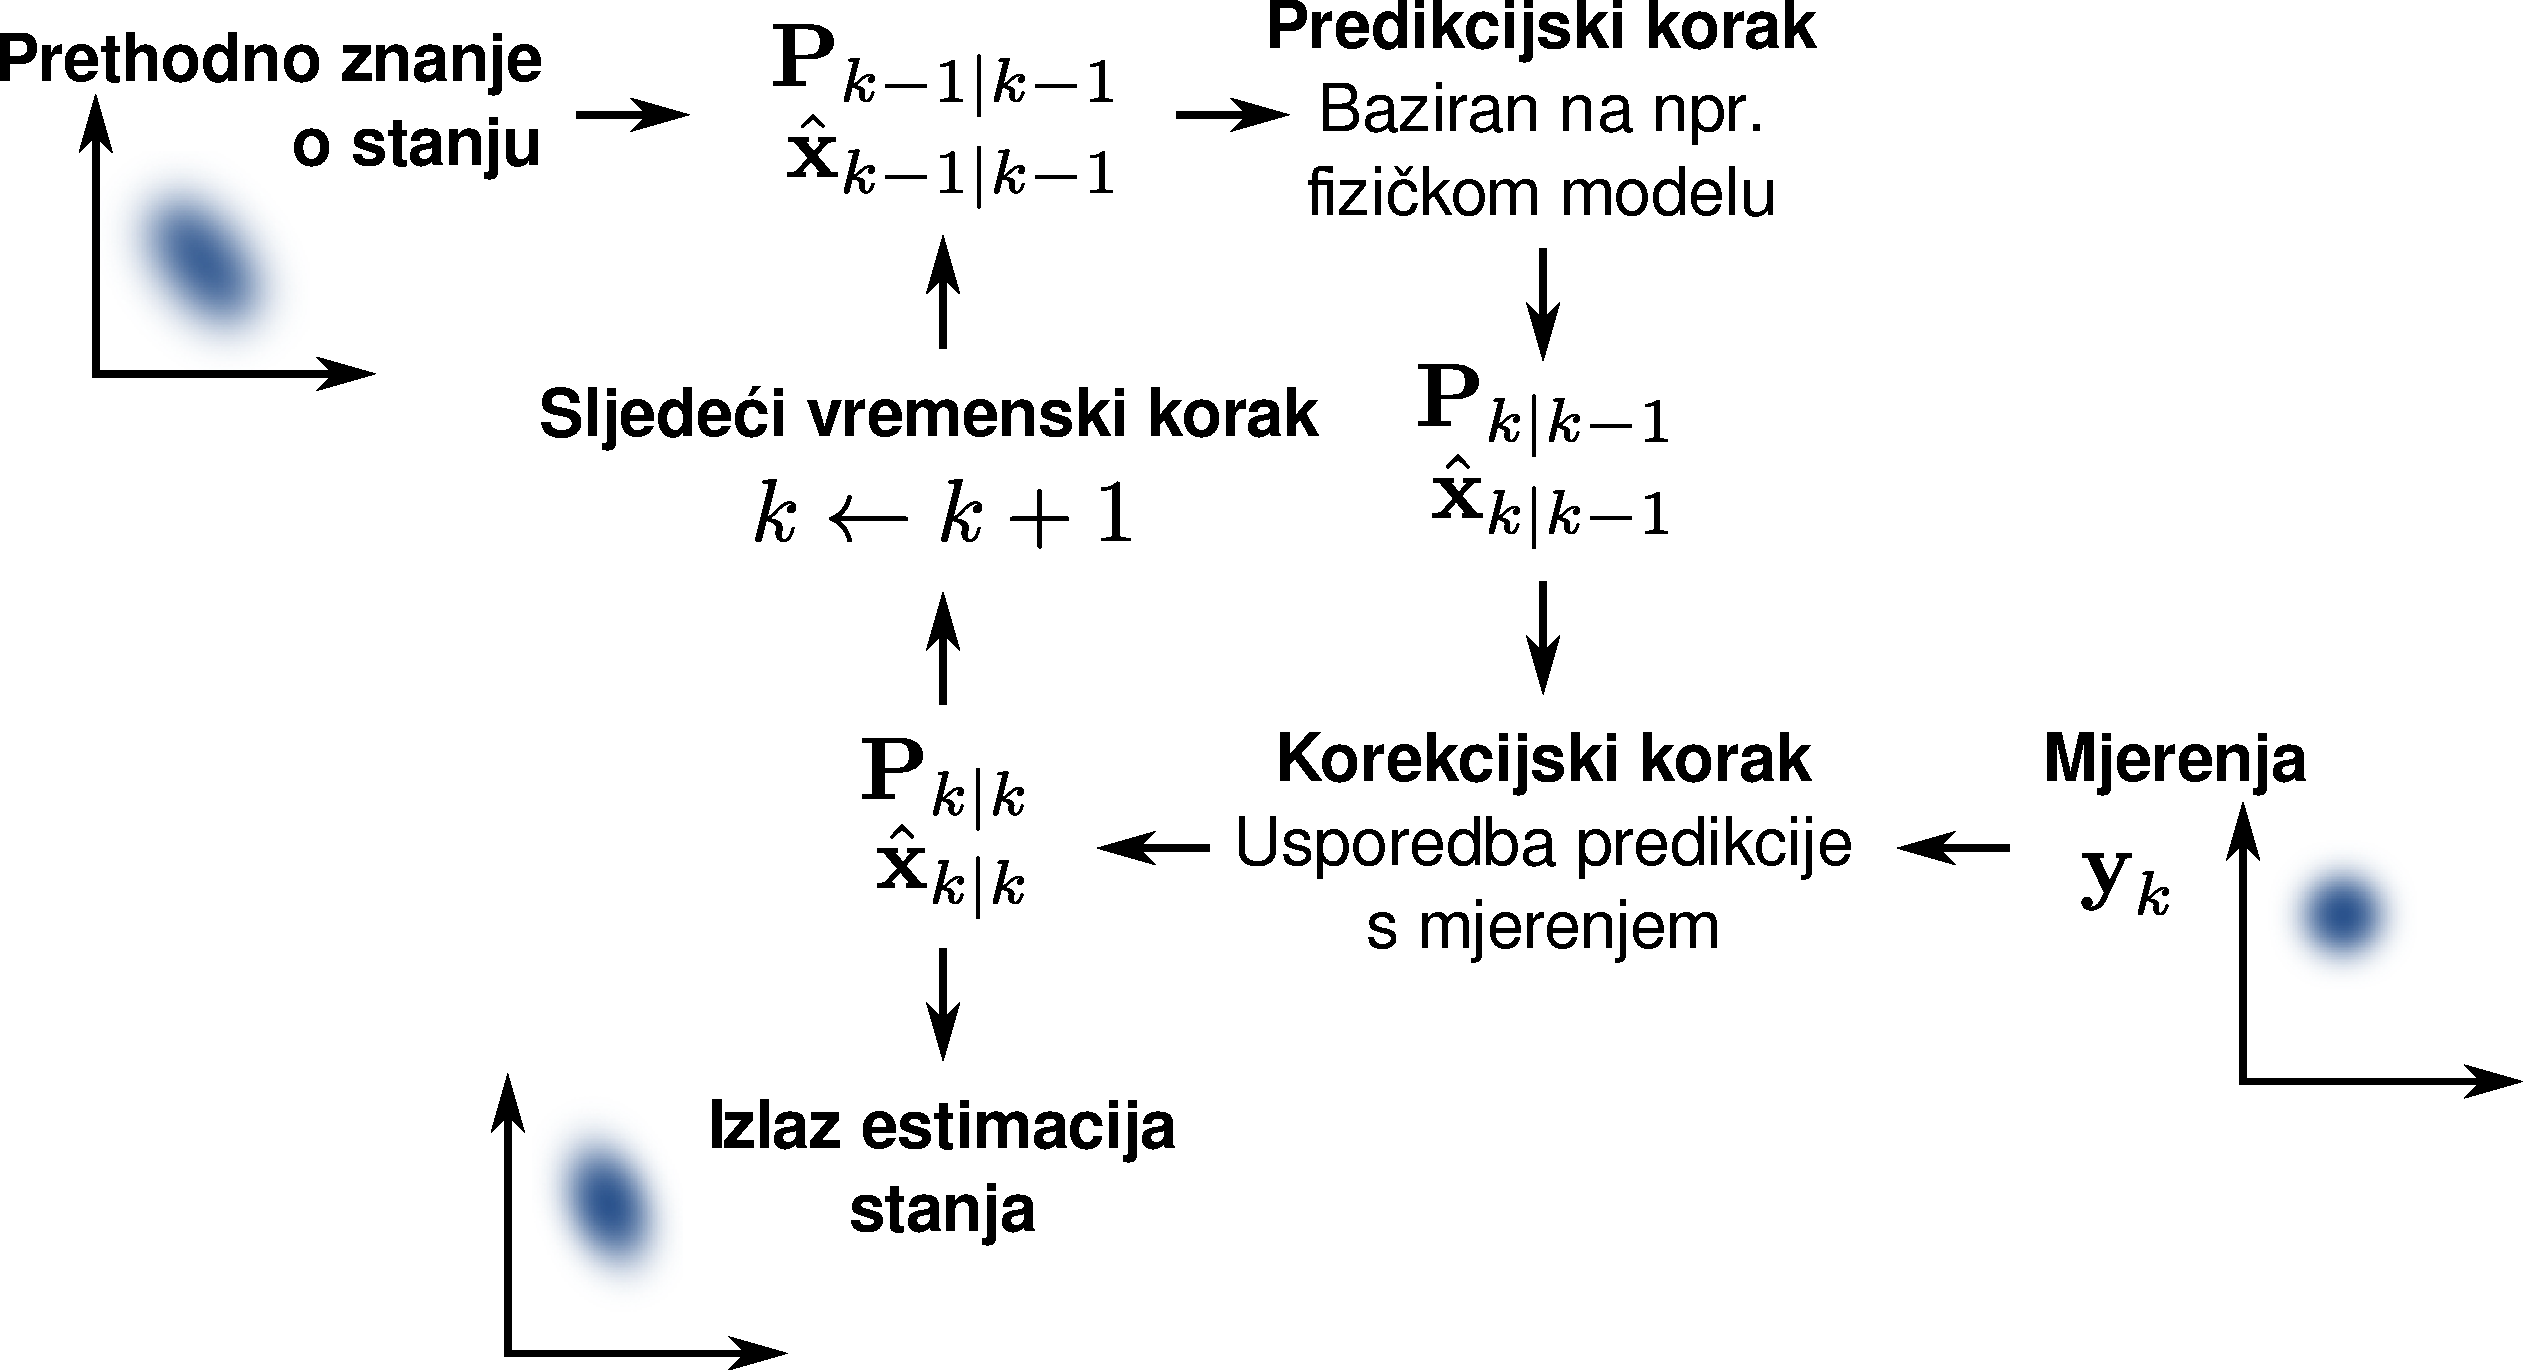
\includegraphics[scale=0.35]{figures/basic-kalman.pdf}
\caption{Osnova Kalmanovog filtra}
\label{fig:basic-kalman}
\end{figure}

\textbf{Prošireni Kalmanov filter} je nelinearna verzija Kalmanovog
filtra gdje promjena stanja i promatrani model ne moraju biti linearne
funkcije.

% subsubsection Proširen Kalmanov filter - EKF (end)

% subsubsection Osnovna ideja  (end)
% subsection Slam (end)

\newpage
\subsection{Poisson algoritam za rekonstrukciju površine} % (fold)
\label{sub:Poisson}
Poisson algoritam za rekonstrukciju površine~\cite{Kazhdan:2006}
razvijen je suradnjom Michaela Kazhdana i Matthewa Bolitha s Johns
Hopkins sveučilišta u Baltimoru i Huguesa Hoppea iz Microsoft Researcha
u Redmondu. Također Kazhdan i Bolitho su implementirali\footnotemark[1]
Poisson algoritam i objavili kod pod BSD licencom. Na osnovu tog rada
algoritam je dodan i u PCL biblioteku.

U ovom potpoglavlju nalazi se osnovna ideja i kratak matematički pregled
algoritma. Opisano je ograničenje algoritma te parametri kojima se može
upravljati rekonstrukcijom površine.

\footnotetext[1]{%
Originalna implementacija Poisson algoritma se nalazi na 
\url{http://www.cs.jhu.edu/~misha/Code/PoissonRecon/Version5.5/}}

% Rekonstrukcija 3D površina iz uzorka točaka je dobro proučavan problem u
% računalnoj grafici. Ona omogućava uklapanje skeniranih
% podataka, ispunjavanje površinskih rupa i ponovnu izgradnju postojećih
% modela.

\subsubsection{Osnovna ideja i kratak matematički pregled} % (fold)
\label{ssub:Osnovna ideja i kratak matematički pregled}

Poisson algoritam pristupa problemu rekonstrukcije površine rješavanjem
Poissonove jednadžbe. To čini upotrebom metode implicitne funkcije.
Točnije računanjem 3D indikacijske funkcije \(\chi\) definirane s 1 u
točkama unutar modela, odnosno s 0 u točkama izvan i dohvaćanjem
rekonstruktruirane površine izvlačenjem odgovarajuće izopovršine.

Algoritam se oslanja na ideju da postoji cjelovita veza između
orijentiranih normala uzetih s površine modela i indikacijske funkcije
modela. Točnije, gradijent indikacijske funkcije je polje vektora koje
je uglavnom popunjeno nulama (jer je indikacijska funkcija uglavnom
konstantna), osim kod točaka blizu površine gdje je jednako unutrašnjim
normalama površine. Stoga, uzorci orijentiranih normala mogu biti
promatrani kao gradijent modela indikacijske funkcije kao što je
prikazano na slici~\ref{fig:poisson-reconstruction.png}

\begin{figure}[h]
\centering
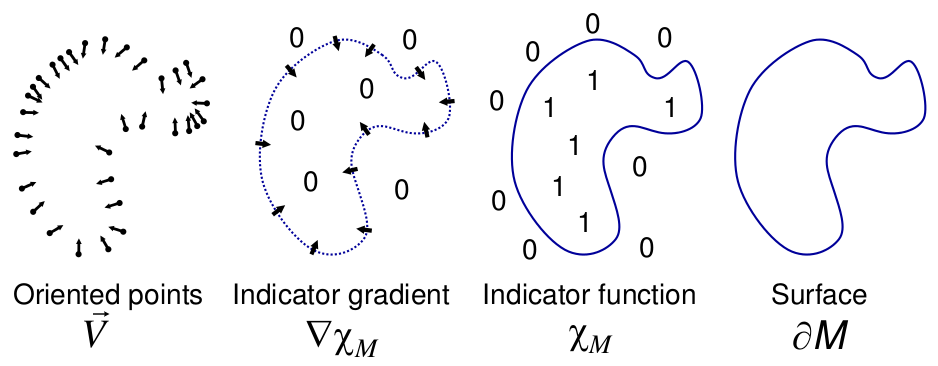
\includegraphics[scale=0.35]{figures/poisson-reconstruction.png}
\caption[]{Prikaz Poisson rekonstrukcije u 2D,
    izvor:~\cite{Kazhdan:2006}}
\label{fig:poisson-reconstruction.png}
\end{figure}

Problem računanja indikacijske funkcije se svodi na invertiranje
operatora gradijenta, odnosno pronalazak funkcije skalara \(\chi\) čiji
gradijent najbolje aproksimira polje vektora \(\vec{V}\) definirano
uzorcima, odnosno 

\begin{equation*}
min_\chi \|\nabla\chi - \vec{V}\|.
\end{equation*}

Ako se primjeni operator divergencije, tada se taj problem pretvara u
standardni Poissonov problem: računanje funkcije skalara \(\chi\) čiji
laplasijan (divergencija gradijenta) je jednak divergenciji polja
vektora \(\vec{V}\),

\begin{equation*}
\Delta \chi \equiv \nabla \cdot \nabla\chi = \nabla \cdot \vec{V}.
\end{equation*}

Predstavljanje rekonstrukciju površine kao Poissonov problem pruža
nekoliko prednosti. Mnoge implicitne metode uklapanja površina
segementiraju podatke u regije za lokalno uklapanje i onda te lokalne
aproksimacije spajaju upotrebom funkcija stapanja. Za razliku od njih,
Poisson rekonstrukcija je globalno rješenje koje razmatra sve podatke
odjednom, bez upotrebe heurstičkih podijela i stapanja. Zbog toga
Poisson rekonstrukcija kreira izrazito glatku površinu koja robusno
aproksimira šumovite podatke.  

Za izvlačenje izopovršine Poisson algoritam koristi Marching Cubes
algoritam~\cite{Lorensen87marchingcubes} koji kreira octree strukturu
podataka za prikaz površine.  Kao što se vidi na
slici~\ref{fig:poisson-marching-cubes.png} Marching Cubes algoritam
dijeli oblak točaka u mrežu voxela marširajući kroz oblak i analizira
koje točke čine izopovršinu objekta.  Detektiranjem koji rubovi voxela
presjecaju izopovršinu modela algoritam kreira mrežu trokuta. Više
informacija o izvlačenju površine se mogu pronaći u radu “Unconstrained
Isosurface Extraction on Arbitrary Octrees” Michaela
Kahzdana~\cite{Kazhdan:2007}

\begin{figure}[h]
\centering
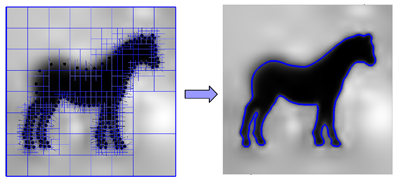
\includegraphics[scale=0.8]{figures/poisson-marching-cubes.png}
\caption[]{Prikaz Marching cubes algoritma, izvor:~\cite{Kazhdan:2007}}
\label{fig:poisson-marching-cubes.png}
\end{figure}

% subsubsection Osnovna ideja i kratak matematički pregled (end)

\subsubsection{Ograničenje Poisson algoritma} % (fold)
\label{ssub:Ograničenje Poisson algoritma}

Ograničenje implementacije Poisson algoritma je u tome što ne uzima u
obzir informacije vezane uz način snimanja oblaka točaka.
Slika~\ref{fig:poisson-buddha.png} pokazuje kip Bude i vidi se primjer takvog
ograničenja. Budući da nema točaka između Budinih nogu, Poisson
algoritam spaja te dvije regije. Algoritam se može unaprijediti
ugradnjom dodatne informacije poput vidokruga i na taj način izbjeći to
ograničenje.


\begin{figure}[h]
\centering
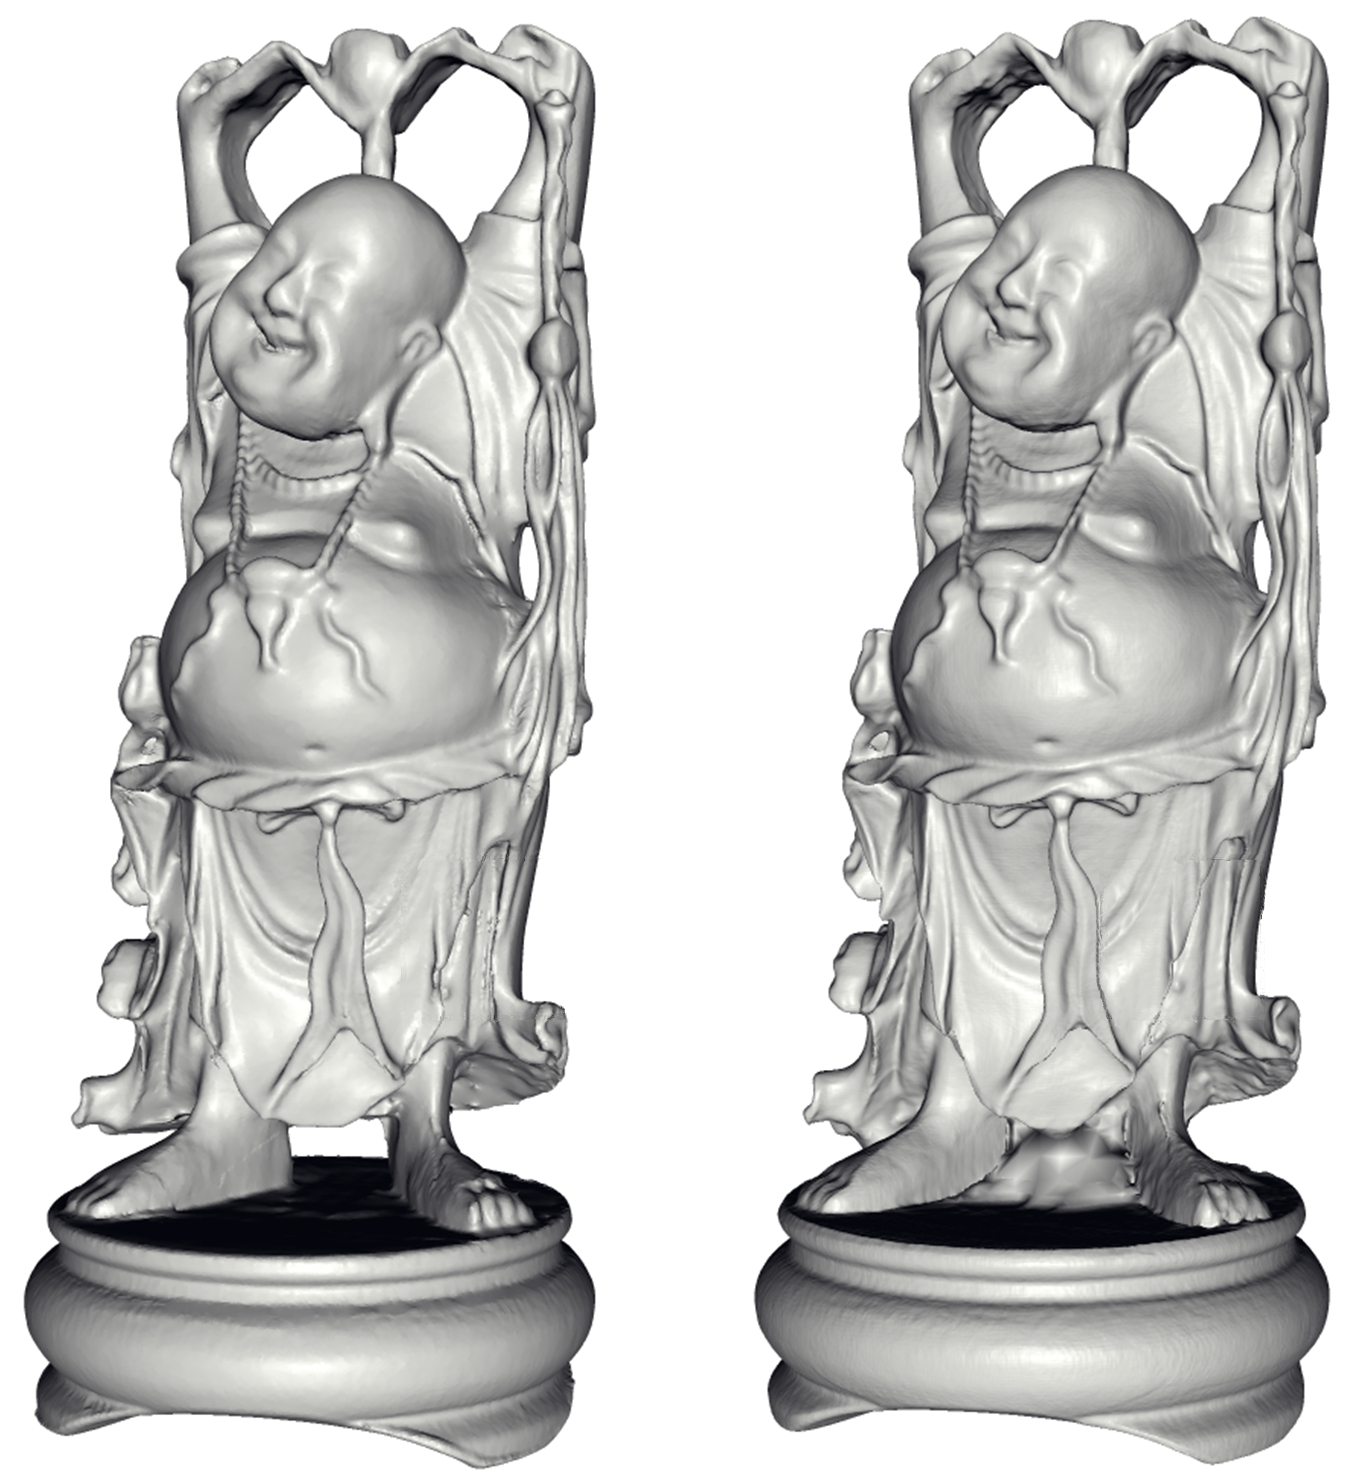
\includegraphics[scale=0.20]{figures/poisson-buddha.png}
\caption[]{Rekonstrukcija modela ``Happy Buddha'' 
VRIP\footnotemark[2] algoritam (lijevo) i Poisson algoritma (desno),
izvor:~\cite{Kazhdan:2006}}
\label{fig:poisson-buddha.png}
\end{figure}

\footnotetext[2]{%
VRIP - Volumetric Range Image Processing~\cite{Curless:1996VRIP}}

% subsubsection Ograničenje Poisson algoritma (end)

\newpage
\subsubsection{Parametri Poisson algoritma} % (fold)
\label{ssub:Parametri Poisson algoritma}
Postoji nekoliko parametara koji utječu na rezultat rekonstrukcije.
\begin{itemize}
    \item \texttt{Depth:} dubina octree stabla koje se koristi za
        rekonstrukciju. Pretpostavljena vrijednost 8.
    \item \texttt{SolverDivide:} postavlja dubinu kod kojeg bloka
        Gauss-Seidel metoda riješava Laplaceovu jednadžbu. Pretpostavljena
        vrijednost 8.
    \item \texttt{IsoDivide:} postavlja dubinu kod kojeg bloka
        ekstraktor izopovršine izvlači izopovršinu. Pretpostavljena vrijednost
        8.
    \item \texttt{SamplesPerNode:} postavlja minimalni broj točaka koje
        se trebaju nalaziti unutar octree čvora kako se octree
        konstrukcija prilagođava gustoći uzorkovanja. Za podatke bez
        šuma 1 - 5, sa šumom 15 - 20. Pretpostavljena vrijednost 1.
    \item \texttt{Scale:} omjer između promjera kocke korištne za
        rekonstrukciju i promjera kocke koja omeđuje uzorke. Pretpostavljena
        vrijednost 1.25.
    \item \texttt{Confidence:} postavljanje zastavice govori
        rekonstruktorciji da koristi veličinu normala kao informaciju o
        pouzdanosti. Ako nije postavljena sve normale se normaliziraju
        prije rekonstrukcije.
\end{itemize}

Od nabrojanih parametara najvažniji utjecaj na generiranu mrežu imaju
\texttt{SamplesPerNode} i \texttt{Depth}. Veća dubina octree stabla
rezultira većom precinosti mreže voxela jer Marching Cubes algoritam
ulazi dublje u stablo. Manja dubina (između 5 i 7) daje glađi model ali
s manje detalja. \texttt{SamplesPerNode} parametar definira koliko će
točaka Marchin Cubes algoritma staviti u jedan čvor rezultantnog octree
stabla. Ako algoritam radi s podacima punim šuma velik uzorak točaka (15
- 20) po čvoru pruža glađenje ali se gube detalji. Dok rad s malim
vrijednostima (1 - 5) održava razinu detalja visokom. Velike vrijednosti
reduciraju kranji broj vrhova poligona, dok male održavaju broj vrhova
visokim.

% subsubsection Parametri Poisson algoritma (end)

% subsection Poisson (end)

% section Tehnologija i teorija (end)

\newpage
\setcounter{figure}{0}

\section{Izgradnja 3D modela scene} % (fold)
\label{sec:Izgradnja 3D modela scene}

\subsection{Snimanje scene 3D kamerom i RGBDSlam programom} % (fold)
\label{sub:Snimanje scene 3D kamerom i RGBDSlam programom}
Program RGBDSlam razvijen je suradnjom
Albert-Ludwigs-Unversität\footnotemark[6] sveučilišta u Freiburgu i
Technische Universität München\footnotemark[7] sveučilišta u Münchenu.
Slobodan je program objavljen pod GPLv3\footnotemark[8] licencom.

\footnotetext[6]{%
\href{http://www.informatik.uni-freiburg.de/~endres/}%
{Felix Endres} i \href{http://www.informatik.uni-freiburg.de/~hess/}%
{Juergen Hess} sa odijela \href{http://ais.informatik.uni-freiburg.de/}%
{Autonomous Intelligent Systems} koji vodi
\href{http://www.informatik.uni-freiburg.de/~burgard/}%
{Prof. Dr. Wolfram Burgard}.
}
\footnotetext[7]{%
\href{http://vision.in.tum.de/members/engelhan}%
{Nikolas Engelhard} sa odijela \href{http://vision.in.tum.de/}%
{Computer Vision Group} koji vodi
\href{http://vision.in.tum.de/members/sturmju}% 
{Dr. Juergen Sturm}.
}
\footnotetext[8]{%
\textit{General Public License version 3} slobodna je licenca koja
osigurava osnovna prava slobodnih programa. Pravo na korištenje,
proučavanje, kopiranje i poboljšavanje. Detaljnije na
\href{http://www.gnu.org/licenses/gpl-3.0.html}% 
{Free Software Foundation} stranicama}

% subsection Snimanje scene 3D kamerom i RGBDSlam programom (end)

\newpage
\subsection{Izgradnja 3D modela scene pomoću mreže trokuta} % (fold)
\label{sub:Izgradnja 3D modela scene pomoću mreže trokuta}

Izgradnja 3D modela scene pomoću mreže trokuta je implementirana u
programu nazvanom \texttt{mesh-reconstruction}.\footnotemark[1]
Program se intenzivno oslanja na biblioteku PointCloud koja je opisana u
potpoglavlju \ref{sub:Biblioteka Pointcloud} Kao što je vidljivo iz
grafikona \ref{fig:flowchart} program je podijeljen u pet osnovnih
funkcija:
\begin{itemize}
    \item Učitavanje oblaka točaka snimljenih RGBDSlam programom.
    \item Reduciranje oblaka točaka.
    \item Uklanjanje pogrešaka pri mjerenju.
    \item Stvaranje i zapisivanje mreže trokuta.
    \item Prikaz mreže trokuta.
\end{itemize}

\footnotetext[1]{%
Program \texttt{mesh-reconstruction} je slobodan program dostupan pod
uvijetima MIT licence. Izvorni kod se nalazi na DVD-u te na web stranici
\href{http://github.com/msvalina/}%
{github.com/msvalina/}}

\begin{figure}[h]
\renewcommand{\figurename}{Grafikon}
\centering
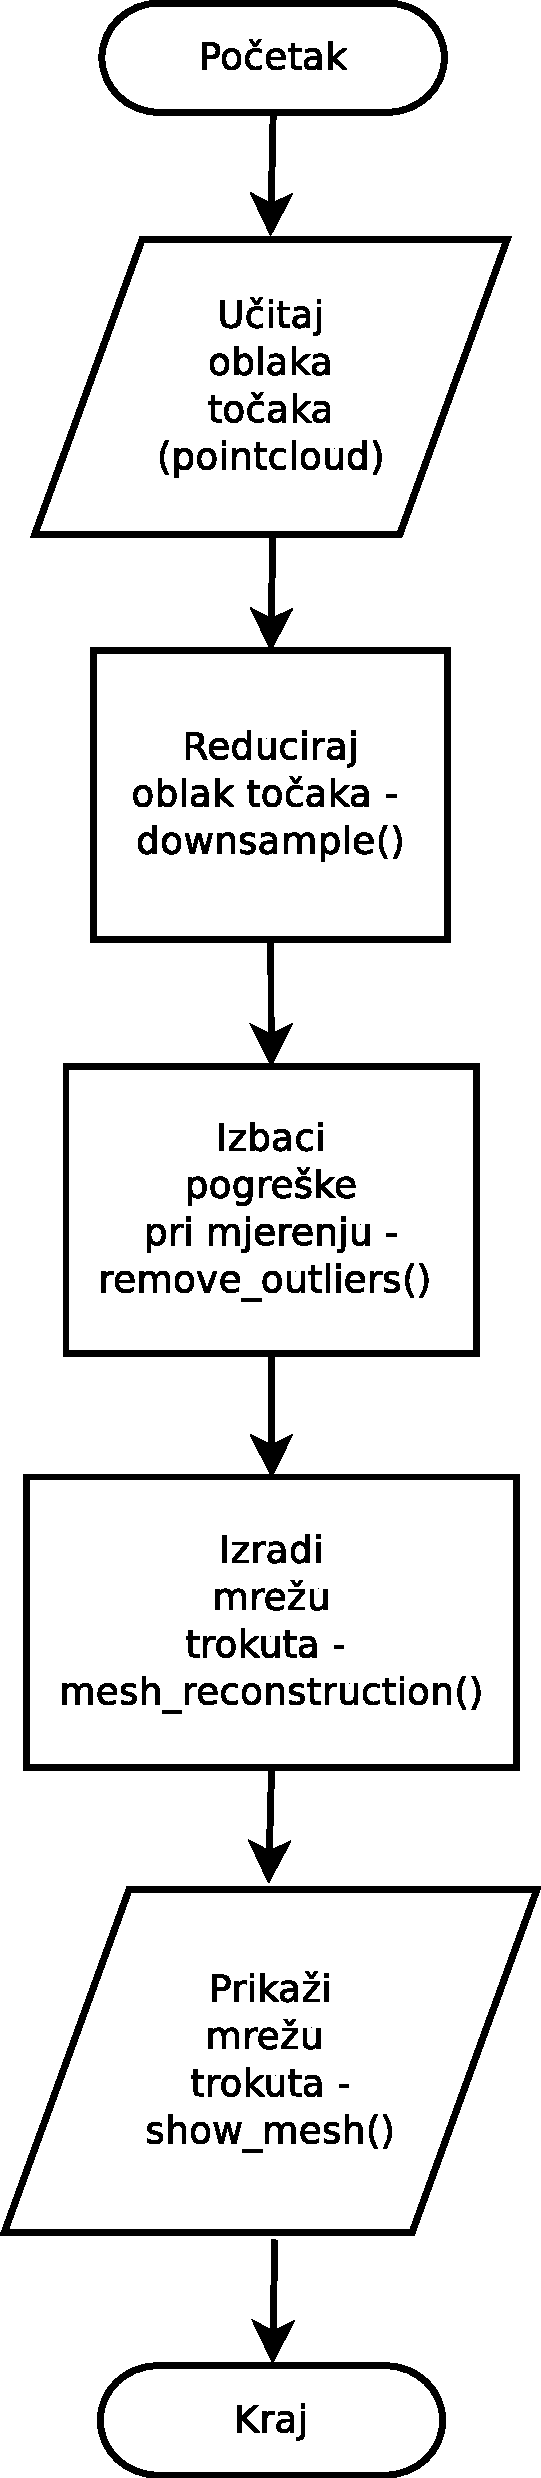
\includegraphics[scale=0.5]{figures/flowchart.pdf}
\caption{Dijagram toka programa \texttt{mesh-reconstruction} }
\label{fig:flowchart}
\end{figure}

U sljedećim potpoglavljima dan je pregled funkcija i PCL klasa na kojima
se baziraju. Također na slici~\ref{fig:running-mesh-reconstruction} se
vidi kako izgleda pokretanje programa, što sve ispisuje na standardni
izlaz te kako prikazuje mrežu trokuta.

\newpage
% Reset counter becouse Grafikon and figures should have diff counters
\setcounter{figure}{0}
\begin{figure}[h]
\centering
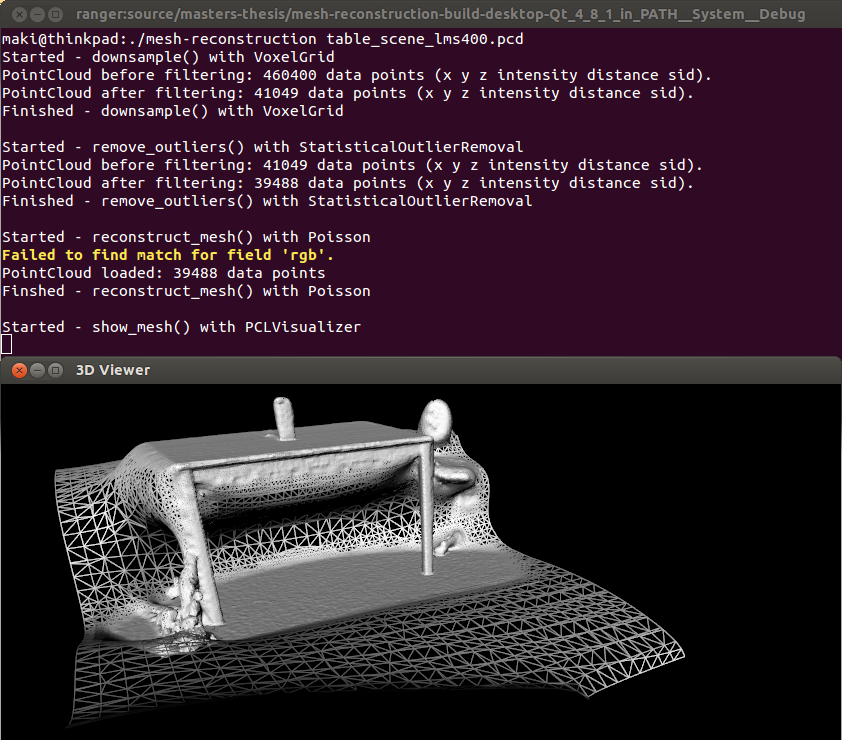
\includegraphics[scale=0.5]{figures/running-mesh-reconstruction.png}
\caption{Prikaz pokretanja programa \texttt{mesh-reconstruction} iz
terminala}
\label{fig:running-mesh-reconstruction}
\end{figure}

\subsubsection{Pregled \texttt{main()} funkcije} % (fold)
\label{ssub:Pregled main funkcije}
\begin{lstlisting}[label=lstMain,caption={Izvorni kod
\texttt{main() funkcije} }]
int main (int argc, char *argv[])
{
    downsample (argc, argv);
    remove_outliers (argc, argv);
    pcl::PolygonMesh mesh_of_triangles;
    reconstruct_mesh (argc, argv, mesh_of_triangles);
    show_mesh (mesh_of_triangles);
    return 0;
}
\end{lstlisting}
Kao što se vidi iz ispisa koda~\ref{lstMain} ideja je da funkcija bude
što manja te da se iz nje samo pozivaju druge funkcije. 

% subsubsection Pregled tt (end)

\newpage
\subsubsection{Učitavanje oblaka točaka} % (fold)
\label{ssub:Učitavanje oblaka točaka}
Program učitava podatke na početku svake funkcije, te ih zapisuje na
izlazu iz funkcije kako bi prije i poslije svake operacije bio dostupan
oblak točaka. Za to koristi \texttt{PCDReader} i \texttt{PCDWriter} klase.
Primjer takvog koda se nalazi u ispisu koda~\ref{lstUcitavanjeOblaka}

\begin{lstlisting}[label=lstUcitavanjeOblaka, caption={Primjer izvornog
koda za učitavanje oblaka točaka}]
    // Init cloud variables 
    pcl::PCLPointCloud2::Ptr cloud (new pcl::PCLPointCloud2());
    pcl::PCLPointCloud2::Ptr cloud_filtered (new pcl::PCLPointCloud2());

    // Fill in the cloud data
    pcl::PCDReader reader;
    reader.read ("pointcloud.pcd", *cloud);
    /* 
     * Do something with cloud
     */
    // Write cloud to a file
    pcl::PCDWriter writer;
    writer.write ("pointcloud-downsampled.pcd",
            *cloud_filtered, Eigen::Vector4f::Zero(),
            Eigen::Quaternionf::Identity(), false);
\end{lstlisting}

% subsubsection Učitavanje oblaka točaka (end)

\subsubsection{Reduciranje oblaka točaka} % (fold)
\label{ssub:Reduciranje oblaka točaka}
Reduciranje obalaka ne unosi bitnih gubitaka informacija, a izvodi se
zbog lakše daljnje obrade oblaka. Izvodi se pomoću \texttt{VoxelGrid}
klase i implementirano je u \texttt{downsample()} funkciji. Dijelovi
funkcije prikazani su u ispisu koda~\ref{lstReduciranje}
\texttt{VoxelGrid} dolazi od riječi \textit{volume pixel grid} i
predstavlja niz malih kocaka u prostoru.

\begin{lstlisting}[label=lstReduciranje, caption={Dio izvornog koda za
reduciranje točaka iz funkcije \texttt{downsample()} }]
    // Create the filtering object
    pcl::VoxelGrid<pcl::PCLPointCloud2> vg;
    vg.setInputCloud (cloud);
    // voxel size to be 1cm^3
    vg.setLeafSize (0.01f, 0.01f, 0.01f);
    vg.filter (*cloud_filtered);
\end{lstlisting}

Kao što se vidi iz ispisa koda~\ref{lstReduciranje} nakon kreiranja
objekta \texttt{vg} predaje mu se oblak točaka nad kojim se vrši
reduciranje. Postavlja se veličina kocke (\textit{voxel}) u našem
slučaju to je 1cm\textsuperscript{3}. Nad tim oblakom prilikom
filtriranja će se kreirati mreža kocaka te će se sve točke unutar jedne
kocke zamjeniti centralnom točkom. Tim postupkom značajno se smanjuje
broj točaka u oblaku kao što je vidljivo iz
slike~\ref{fig:tablescene-downsample}

\begin{figure}[h]
\centering
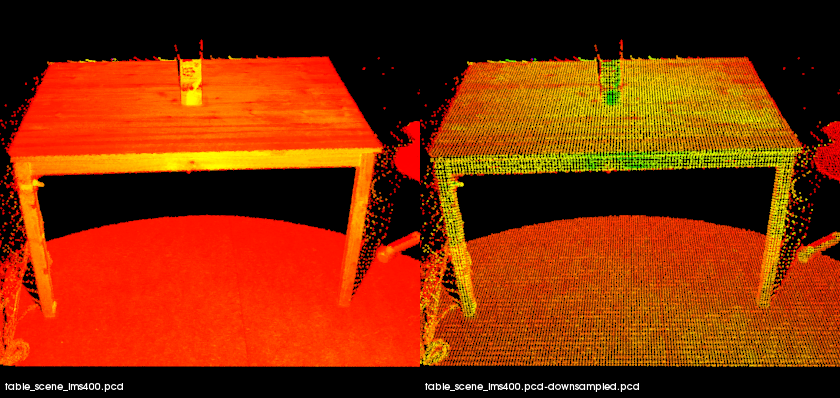
\includegraphics[scale=0.5]{figures/tablescene-downsampling-example.png}
% If there is \footnote in caption brackets [] must be used
\caption[description for List of Figures]{%
    Oblak točaka \textit{table\_scene}\footnotemark[2] prije i poslije %
    \texttt{downsample()} funkcije}
\label{fig:tablescene-downsample}
\end{figure}

\footnotetext[2]{Oblak točaka \texttt{table\_scene\_lms400.pcd} je
objavljen pod uvijetima BSD licence - 
\href{https://github.com/PointCloudLibrary/data/blob/master/tutorials%
/table\_scene\_lms400.pcd}{izvor}}

% subsubsection Reduciranje oblaka točaka (end)

\subsubsection{Uklanjanje pogrešaka pri mjerenju} % (fold)
\label{ssub:Uklanjanje pogrešaka pri mjerenju}
Šum pri mjerenju je sastavni dio svakog mjernog uređaja pa tako i
Kineckt kamere. PointCloud biblioteka ima ugrađenu
\texttt{StatisticalOutlierRemoval} klasu koja uklanja šum a 
implementirana je u funkciji \texttt{remove\_outlieres()}.
Iz ispisa koda~\ref{lstUklanjanje} se vidi kako se klasa koristi.

% minipage ensures that listing won't be split between pages
% but it seams like it's pushing whole box slightly to the right
% \begin{minipage}{\textwidth}
\begin{lstlisting}[label=lstUklanjanje, caption={Dio izvornog koda 
iz funkcije \texttt{remove\_outliers()} }]
    // Create the filtering object
    pcl::StatisticalOutlierRemoval<pcl::PCLPointCloud2> sor;
    sor.setInputCloud (cloud);
    // Set number of neighbors to analyze
    sor.setMeanK (50);
    sor.setStddevMulThresh (1.0);
    sor.filter (*cloud_filtered);
\end{lstlisting}
% \end{minipage}

Nakon kreiranja objekta \texttt{sor} i predavanja oblaka postavljena su
još dva parametra. Prvi \texttt{setMeanK} je broj susjednih točaka koje
će filter analizirati. Drugi \texttt{setStddevMulThresh} pak kaže da će
sve točke u okolini ispitane točke čije su udaljenosti veće od jedne
standardne devijacije očekivane udaljenosti biti označne kao šum
(\textit{outlier}) i odbačene. Rezultati rada funkcije se vide na
slici~\ref{fig:tablescene-outliers}

\begin{figure}[h]
\centering
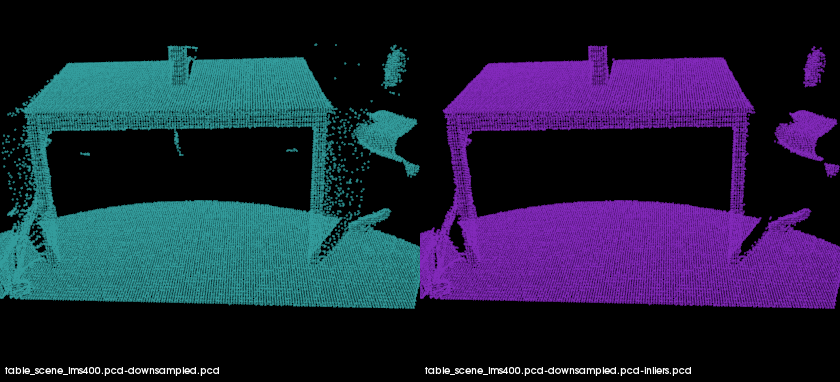
\includegraphics[scale=0.5]{figures/tablescene-remove-outliers-example.png}
\caption{Oblak točaka: lijevo poslije \texttt{downsample()} i desno poslije
\texttt{remove\_outliers()} }
\label{fig:tablescene-outliers}
\end{figure}

% subsubsection Uklanjanje pogrešaka pri mjerenju (end)

\newpage
\subsubsection{Stvaranje i zapisivanje mreže trokuta} % (fold)
\label{ssub:Stvaranje i zapisivanje mreže trokuta}

Nakon pripreme oblaka točaka funkcijama \texttt{downsample()} i
\texttt{remove\_outliers()} slijedi stvaranje mreže trokuta unutar
funkcije \texttt{mesh\_reconstruction()}. Stvaranje mreže trokuta se
može podijeliti u tri koraka. Prvi je estimiranje normala nad oblakom
točaka. Drugi je spajanje estimiranih normala i oblaka točaka u
zajedniči oblak točaka s normalama. Treći korak je pozivanje algoritma
za stvaranje mreže nad novo stvorenim oblakom.

\begin{lstlisting}[label=lstStvaranje1, caption={Dio izvornog koda iz
funkcije \texttt{reconstruct\_mesh()} }]
    // Normal estimation
    pcl::NormalEstimation<PointType, Normal> normEst;
    pcl::PointCloud<Normal>::Ptr normals (new pcl::PointCloud<Normal>);
    
    // Create kdtree representation of cloud, 
    // and pass it to the normal estimation object. 
    pcl::search::KdTree<PointType>::Ptr tree (new
            pcl::search::KdTree<PointType>);
    tree->setInputCloud (cloud);
    normEst.setInputCloud (cloud);
    normEst.setSearchMethod (tree);
    // Use 20 neighbor points for estimating normal
    normEst.setKSearch (20);
    normEst.compute (*normals);
\end{lstlisting}

Iz ispisa koda~\ref{lstStvaranje1} se vidi da je prije estimiranja
normala nad oblakom točaka potrebno inicijalizirati objekt za
spremanje normala i za estimaciju. Nakon toga definira se
stablo za pretraživanje oblaka tipa \texttt{KdTree}.\footnotemark[3]
Stablu se tada predaje oblak za pretraživanje. Objektu za
estimaciju \texttt{normEst} tada se predaje oblak i stablo te broj
susjednih točaka nad kojima se vrši estimacija
normala\footnotemark[4]. 

\footnotetext[3]{%
K dimenzionalno stablo je detaljno objašnjeno na stranici \href{http://%
pointclouds.org/documentation/tutorials/kdtree\_search.php}%
{pointclouds.org/documentation}}
\footnotetext[4]{%
Estimacija normala detaljno je objašnjena na stranici \href{http://%
pointclouds.org/documentation/tutorials/normal\_estimation.php}%
{pointclouds.org/documentation}}

Nakon estimacije normala slijedi spajanje estimiranih normala i oblaka u
novi oblak točaka s normalama. Kao što je prikazano u ispisu
koda~\ref{lstStvaranje2} Taj oblak točaka je prikazan na 
slici~\ref{fig:tablescene-normals}

\newpage
\begin{lstlisting}[label=lstStvaranje2,caption={Dio izvornog koda iz
funkcije \texttt{reconstruct\_mesh()} }]
    // Concatenate the XYZ and normal fields
    pcl::PointCloud<PointTypeN>::Ptr cloud_with_normals (new
            pcl::PointCloud<PointTypeN>);
    pcl::concatenateFields (*cloud, *normals, *cloud_with_normals);
    // cloud_with_normals = cloud + normals

    // Create search tree 
    pcl::search::KdTree<PointTypeN>::Ptr tree2 (new
            pcl::search::KdTree<PointTypeN>);
    tree2->setInputCloud (cloud_with_normals);

    // Initialize objects 
    // psn - for surface reconstruction algorithm
    // triangles - for storage of reconstructed triangles
    pcl::Poisson<PointTypeN> psn;
    pcl::PolygonMesh triangles;

    psn.setInputCloud(cloud_with_normals);
    psn.setSearchMethod(tree2);
    psn.reconstruct (triangles);
    psn.setOutputPolygons(false);
\end{lstlisting}

Nad stvorenim oblakom s normalama stvara se stablo za pretraživanje.
Zatim se inicijaliziraju objekti \texttt{psn} i \texttt{triangles}.
\texttt{psn} predstavlja \texttt{Poisson}\footnotemark[5] algoritam za
stvaranje mreže trokuta. \texttt{triangles} je objekt tipa
\texttt{PolygonMesh} za spremanje izračunatih koordinata trokuta.
Algoritmu se sada predaje ulazni oblak, stablo pretraživanja i poziva se
rekonstrukcija.

\footnotetext[5]{%
Poisson algoritam su razvili Michael Kazhdan i Matthew Bolitho,
objavljen je pod BSD licencom. \href{http://www.cs.jhu.edu/~misha/Code/%
PoissonRecon/Version5.5/}{Službena stranica.}}

\begin{figure}[h]
\centering
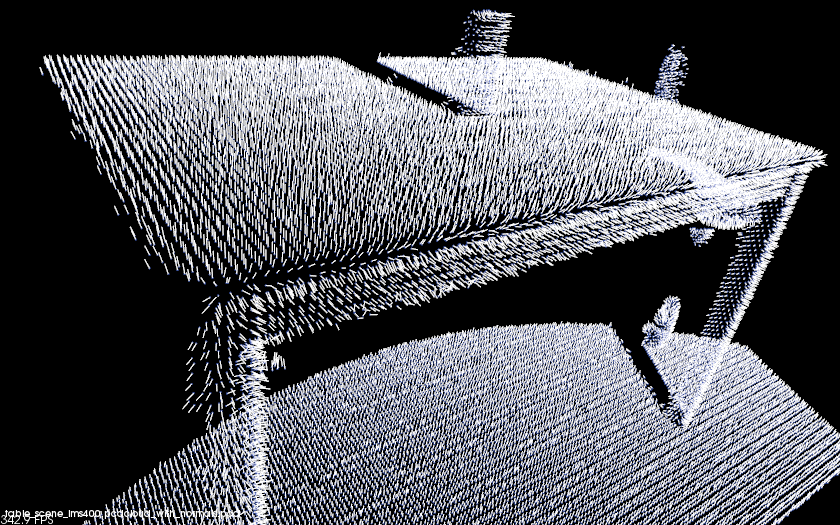
\includegraphics[scale=0.5]{figures/tablescene-normals.png}
\caption{Prikaz oblaka točaka \texttt{tablescene} s estimiranim
normalama }
\label{fig:tablescene-normals}
\end{figure}

Ispis koda~\ref{lstStvaranje3} prikazuje korištenje klase
\texttt{saveVTKFile} za spremanje objekta \texttt{triangles} u datoteku
s vtk ekstenzijom.

\begin{lstlisting}[label=lstStvaranje3,caption={Dio izvornog koda iz
funkcije \texttt{reconstruct\_mesh()} }]
    // Write reconstructed mesh
    if (argc < 2){
        pcl::io::saveVTKFile
            ("pointcloud-downsampled-outliers-mesh.vtk",
             triangles);
    }
    else {
        std::string str;
        str.append(argv[1]).append("-mesh.vtk");
        pcl::io::saveVTKFile (str, triangles);
    }
\end{lstlisting}

% subsubsection Stvaranje i zapisivanje mreže trokuta (end)

\subsubsection{Prikazivanje mreže trokuta} % (fold)
\label{ssub:Prikazivanje mreže trokuta}
Prikazivanje mreže trokuta omogućava \texttt{PCLVisualizer} klasa. Ista
klasa se koristi u komandono linijskom programu za prikaza oblaka točaka
\texttt{pcl\_vieweru}. U ispisu koda~\ref{lstPrikaz} se vidi
jednostavnost upotrebe klase. Nakon kreiranja objekta \texttt{viewer} i
postavljanja parametara poziva se beskonačna petlja unutar koje se
pokrene prozor s prikazom mreže trokuta. Klikom na tipku \texttt{q}
izlazi se iz petlje i program završava.
Slika~\ref{fig:tablesecne-mesh-perspectives} prikazuje izgled mreže iz
četiri pogleda.

\begin{figure}[h]
\centering
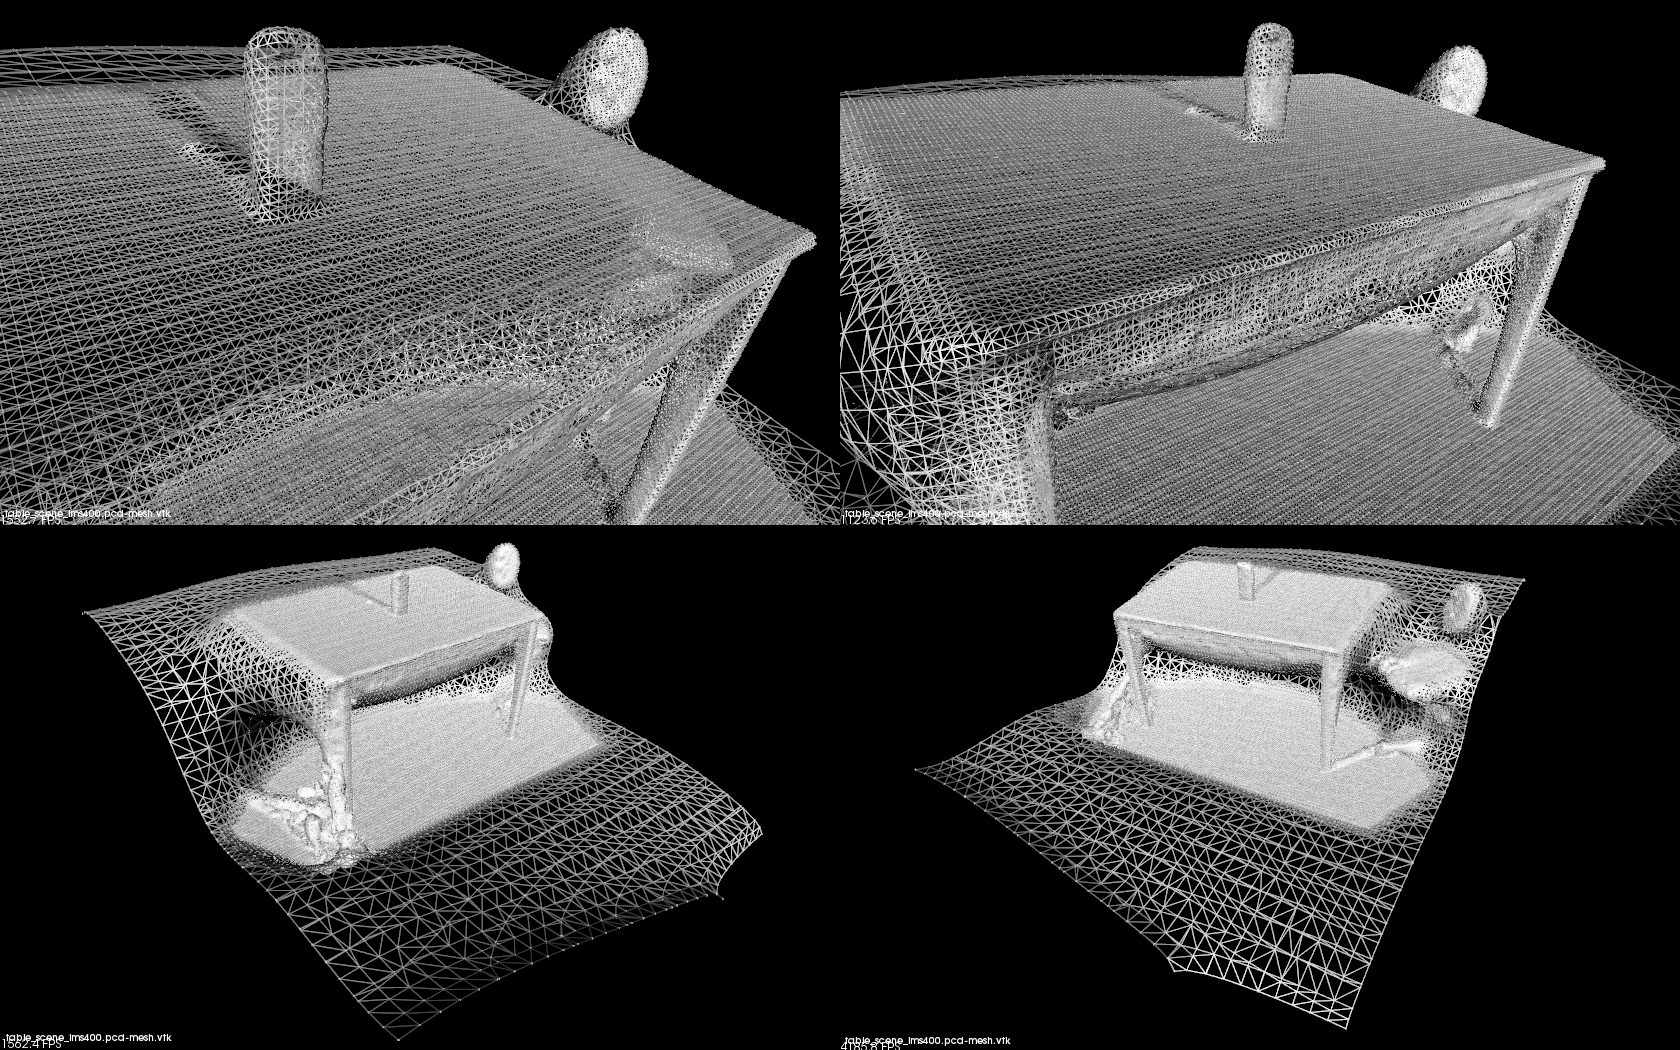
\includegraphics[scale=0.25]{figures/tablescene-mesh-perspectives.png}
\caption{Prikaz mreže trokuta funkcijom \texttt{show\_mesh()} }
\label{fig:tablesecne-mesh-perspectives}
\end{figure}

\newpage
\begin{lstlisting}[label=lstPrikaz,caption={Izvorni kod funkcije
\texttt{show\_mesh()} }]
void show_mesh (const pcl::PolygonMesh& mesh_of_triangles)
{
    std::cout << "Started - show_mesh() with PCLVisualizer\n";
    // Create viewer object and show mesh
    boost::shared_ptr<pcl::visualization::PCLVisualizer> viewer (new
          pcl::visualization::PCLVisualizer ("3D Viewer"));
    viewer->setBackgroundColor (0, 0, 0);
    viewer->addPolygonMesh (mesh_of_triangles, "sample mesh");
    viewer->initCameraParameters (); 
    while (!viewer->wasStopped ())
    {
        viewer->spinOnce (100); boost::this_thread::sleep
            (boost::posix_time::microseconds (100000));
    }
    std::cout << "Finshed - show_mesh() with PCLVisualizer\n";
}
\end{lstlisting}


% subsubsection Prikazivanje mreže trokuta (end)

% subsection Izgradnja 3D modela scene pomoću mreže trokuta (end)

% section Izgradnja 3D modela scene (end)

\newpage
\setcounter{figure}{0}

\section{Rezultati} % (fold)
\label{sec:Rezultati}

Tijekom izrade diplomskog rada snimljeno je šest scena upotrebom
programa RGBDSlam i iz tih snimaka (slika~\ref{fig:01-all.png}) su
izgrađeni 3D modeli objekata i scena pomoću programa
\texttt{mesh-reconstruction}. Sve snimke i izrađeni modeli nalaze se na
priloženom DVDu. U ovom poglavlju su prikazani rezultati izgradnje i
ispitana je funkcionalnost izgradnje 3D modela scena pomoću 3D kamere.
Za ispitivanje funkcionalnosti metode odabrane su tri scene:
etfos-ured-2013-07-30, etfos-hol-2013-11-20, etfos-hodnik-11-27. Prije
prikaza rezultata potrebno je istaknuti nekoliko problema odnosno
ograničenja ove metode.

Problemi sa načinom stjecanja oblaka točaka
Problemi sa izgradnjom 3D modela 

\begin{figure}[h]
\centering
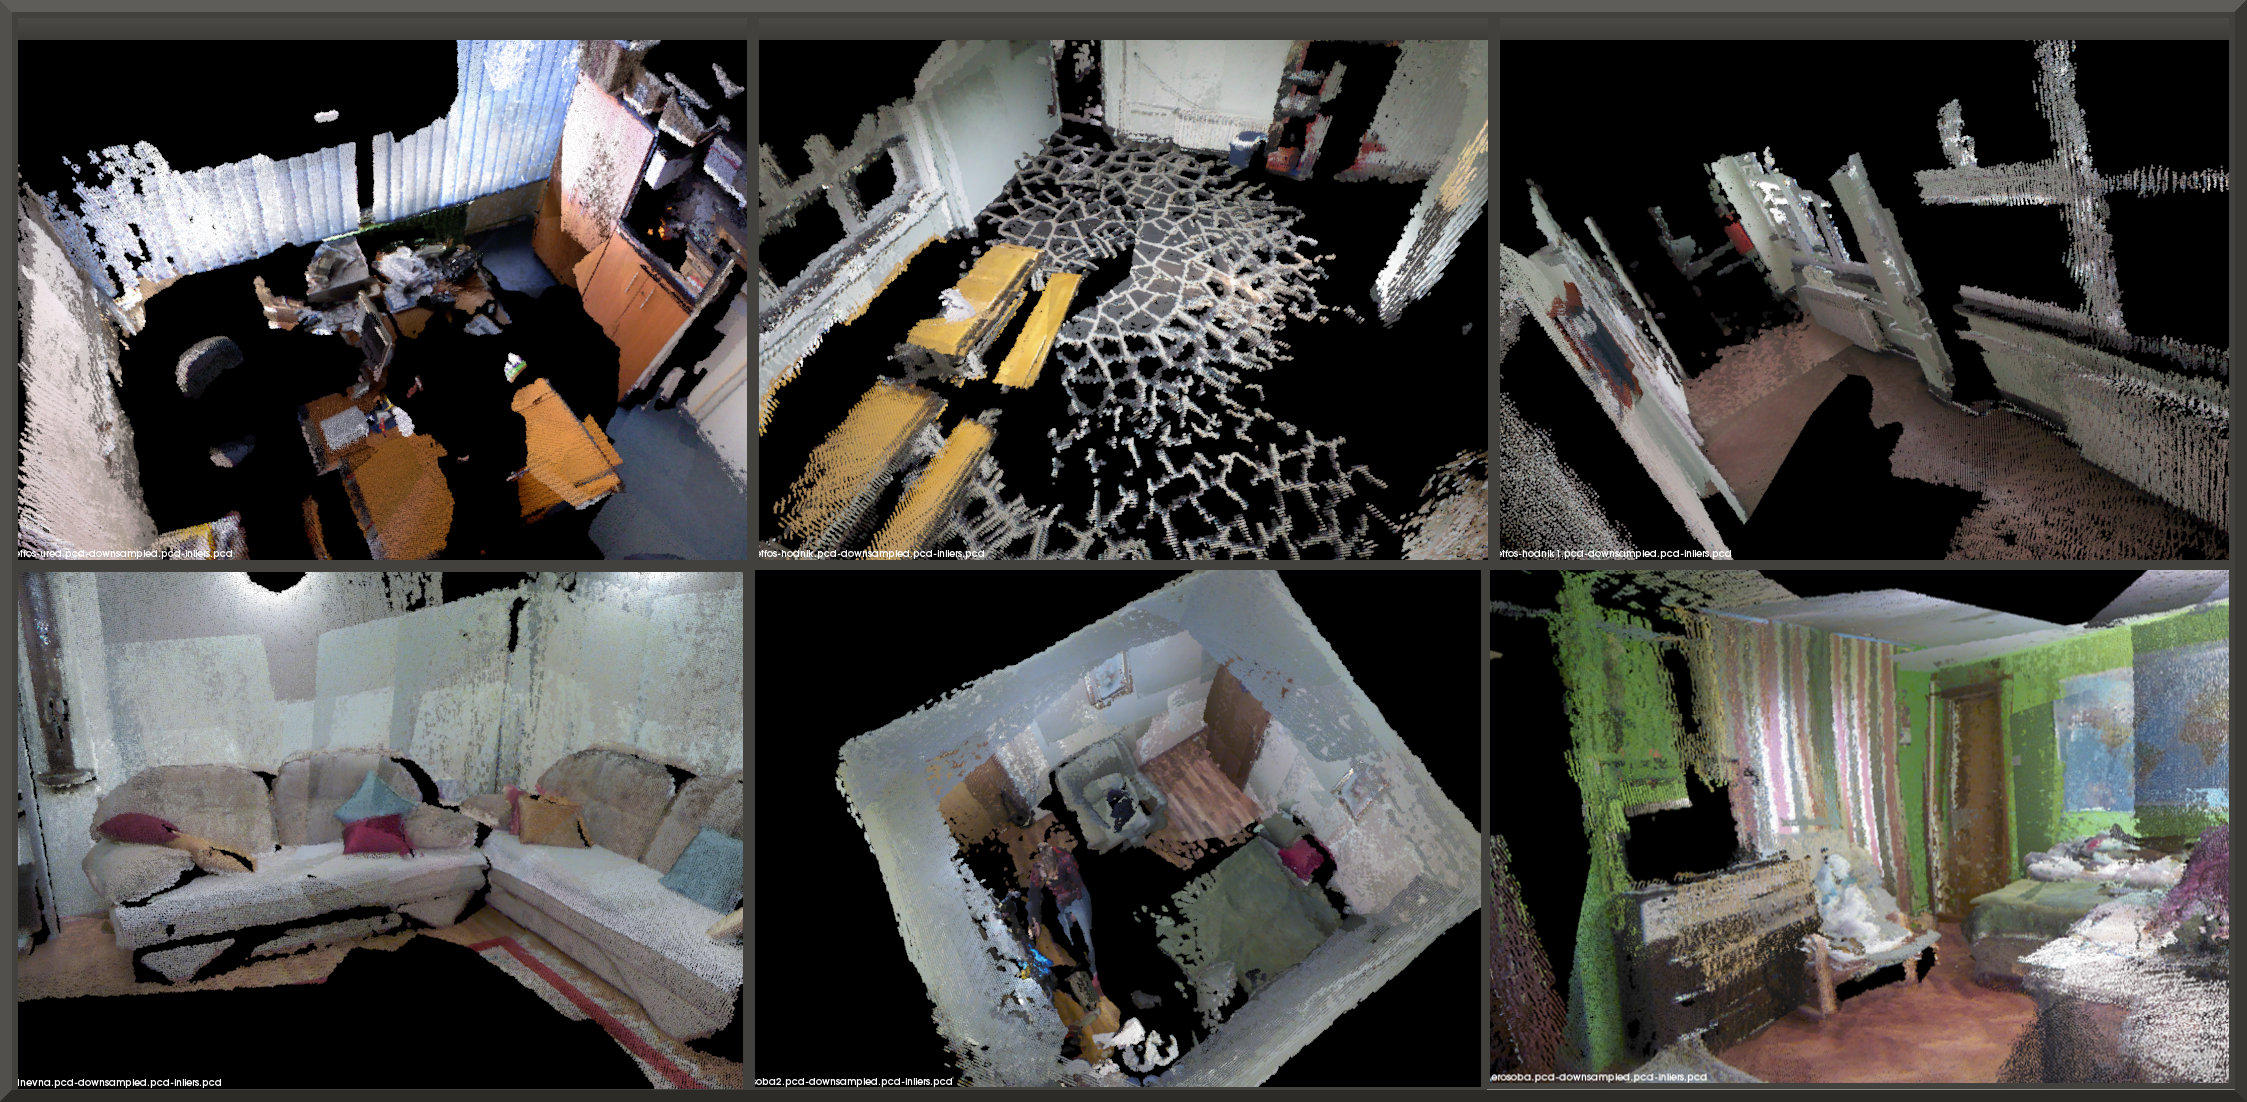
\includegraphics[scale=0.15]{figures/01-all-pcd.png}
\caption{Prikaz svih snimljenih scena}
\label{fig:01-all.png}
\end{figure}

\newpage
\subsection{Prikaz izgrađenih modela scena i objekata} % (fold)
\label{sub:Prikaz izgradenih modela scena i objekata}

\textbf{Snimka: Etfos ured 2013-07-30} 

\begin{figure}[h]
\centering
\includegraphics[scale=0.25]{figures/02-etfos-ured-vtk-pcd-all.png}
\caption{Prikaz izrađenog modela i snimljenog oblaka točaka}
\label{fig:02-etfos-ured-vtk-pcd.png}
\end{figure}

% subsection Prikaz izgrađenih modela scena i objekata (end)

% section Rezultati (end)


\newpage
\setcounter{figure}{0}

\section{Zaključak} % (fold)
\label{sec:Zaključak}

U ovom diplomskom radu razvijen je i predstavljen program za izgradnju
mreže trokuta mesh-reconstruction. Program se upotrebljava nad oblakom
točaka prikupljenim RGBDSlam programom. Ispitana je funkcionalnost i
kvaliteta postupka snimanjem i izgradnjom nekoliko 3D modela scena
pomoću 3D kamere. Tijekom izrade rada pojavilo se niz prepreka koje je
trebalo riješiti da bi se došlo do upotrebljivog programa. Glavne
prepreke su bile prevođenje, instalacija, proučavanje i pokretanja
programa RGBDSlam te postavljanje radne okoline za pisanje programa. 

Predstavljeni postupak snimanja i izgradnje 3D modela ima svoje
prednosti i nedostatke. Nedostatci su vezani uz ograničenja korištenih
tehnologija i algoritama. Npr. snimanje Kinectom ograničeno je na
prostore u unutrašnjosti, uspješnost snimanja RGBDSlam programom uvelike
ovisi o detekciji i sparivanju značajki, Poisson algoritam ne uzima u
obzir informaciju o boji itd. Prednosti je svakako nabavna cijena
kamere koja se može nabaviti za manje od tisuću kuna. Isto tako svi
korišteni programi objavljeni su pod slobodnim licencama te su dostupni
za proučavanje, poboljšavanje i upotrebu u bilo koje svrhe.  

Postoji potencijal opisanog postupka izgradnje odnosno generalna ideja
ima značajne mogućnosti buduće primjene. Sve veća dostupnost 3D printera 
na tržištu stvara potražnju za jednostavnim i jeftinim
rješenjem skeniranja 3D scena i objekata. Osim toga dizajneri FPS (engl.
\textit{First Person Shooter}) igara mogli bi koristiti sličan postupak
za skeniranje prostorija od kojih bi izgrađivali 3D modele.

Mogućnosti za poboljšanja postoje na svim razinama. Najveći utjecaj na
krajnje rezultate bilo bi proširivanje Poisson algoritma logikom za
očuvanje informacije o boji. Isto tako algoritamu bi se mogla dodati
logika koja uklanja zatvaranje velikih rupa, ideja je da se prođe još
jednom kroz izrađenu mrežu te pronađu i odbace veliki trokuti. Kod
snimanja scene jednostavno poboljšanje bilo bi korištenje jačeg računala
i automatskog snimanja. Najzahtjevniji je, mehanizam zatvaranja petlje o
kojemu značajno ovisi kvaliteta rezultata. To je još uvijek predmet
intenzivnog istraživanja. 

% section Zaključak (end)

\newpage
% Removing page numbering from this page but not from showing up on TOC
\thispagestyle{empty}
\begin{thebibliography}{9}

\bibitem{lamport94}
  Leslie Lamport,
  \emph{\LaTeX: A Document Preparation System}.
  Addison Wesley, Massachusetts,
  2nd Edition,
  1994.

\end{thebibliography}

\newpage

\section{Sažetak} % (fold)
\label{sec:Sažetak}

% section Sažetak (end)

\newpage

\section*{Životopis} % (fold)
\addcontentsline{toc}{section}{Životopis}
\label{sec:Životopis}

% section Životopis (end)

\newpage
\thispagestyle{empty}

\section*{Prilozi} % (fold)
\addcontentsline{toc}{section}{Prilozi}
\label{sec:Prilozi}

\subsection*{Prevođenje i instalacija RGBDSlam programa} % (fold)
\label{sub:RGBDSlam prilog}

Prevođenje i instalacije programa rađena je na Ubuntu 12.04 GNU/Linux
distribuciji pomoću skripte prikazane u ispisu~\ref{skripta} Upute za
ostale distribucije se nalaze na \url{http://wiki.ros.org/rgbdslam}.
Skripta automatizira dodavanje ROS repozitorija i poziva instalaciju
svih potrebinh paketa. Zatim postvlja ROS varijable okruženja potrebne za
pokretanje RGBDSlam programa. Tada se klonira izvorni kod programa i
pozivaju naredbe za instaliranje i prevođenje programa.

\begin{lstlisting}[language=bash,label=skripta, keywords={sudo, wget, 
    echo, apt-get, rosdep, roscd, rosmake}, caption={Ispis shell skripte 
    za instalaciju rgbdslam programa}]
# Better pick a mirror close to you. 
# See http://ros.org/wiki/ROS/Installation/UbuntuMirrors
sudo sh -c '. /etc/lsb-release && echo "deb http://packages.ros.org/ros/ubuntu $DISTRIB_CODENAME main" > /etc/apt/sources.list.d/ros-latest.list' 

wget http://packages.ros.org/ros.key -O - | sudo apt-key add -

sudo aptitude update

# This will draw gigabytes from the network:
sudo apt-get install ros-fuerte-perception-pcl ros-fuerte-vision-opencv ros-fuerte-octomap-mapping python-rosdep 
sudo apt-get install ros-fuerte-openni-launch

echo 'source /opt/ros/fuerte/setup.bash' >> ~/.bashrc
echo 'export ROS_PACKAGE_PATH=~/ros:$ROS_PACKAGE_PATH' >> ~/.bashrc
. ~/.bashrc

svn co http://alufr-ros-pkg.googlecode.com/svn/trunk/rgbdslam_freiburg ~/ros/rgbdslam_freiburg

sudo rosdep init
rosdep update
rosdep install rgbdslam_freiburg
roscd rgbdslam

# This will take a while:
rosmake rgbdslam_freiburg
\end{lstlisting}


% subsection RGBDSlam prilog (end)

% section Prilozi (end)


\end{document}
